\protect\hypertarget{titlepage.xhtml}{}{}

\protect\hypertarget{index_split_000.html}{}{}

NO. 6 \textbar{} Atsuko Asano

\protect\hypertarget{index_split_002_split_000.html}{}{}

\hypertarget{index_split_002_split_000.htmlux5cux23calibre_pb_0}{%
\subsection{Volume
8}\label{index_split_002_split_000.htmlux5cux23calibre_pb_0}}

\protect\hypertarget{index_split_002_split_001.html}{}{}

\emph{You don't feel it?}

\emph{Feel? Feel what?}

\emph{Something off.}

\hypertarget{index_split_002_split_001.htmlux5cux23calibre_pb_1}{}

\hypertarget{index_split_002_split_001.htmlux5cux23calibre_pb_0}{}

\protect\hypertarget{index_split_002_split_002.html}{}{}

\hypertarget{index_split_002_split_002.htmlux5cux23calibre_toc_2}{%
\subsection{CHAPTER
1}\label{index_split_002_split_002.htmlux5cux23calibre_toc_2}}

\subsubsection{Ring the alarum bell!}

\emph{I gin to be aweary of the sun,}

\emph{And wish the estate o' the world were now undone.}

\emph{Ring the alarum bell! Blow, wind! come, wrack!}

\emph{At least we'll die with harness on our back.~}

\emph{- Macbeth, Act V Scene V}

I love you, Shion. I love you more than anyone else.

Brains floated in the middle of the transparent columns.

Human brains.

How many? Ten, twenty, thirty... perhaps more than fifty. There seemed
to be a light source at the base of the column, for the entirety of it
emitted a soft, white glow.

A scene he had never seen before. It was orderly, inorganic, and
sterile. Not a single stain marred the smooth floor. The chamber was
odourless and almost soundless. But that in itself was terrifying. Shion
felt that this scene was more terrifying than any he had seen until now.
He couldn't hear the tearful cries, the screams, or groans. There were
no corpses, no flowing blood, no faces distorted in agony. But this
scene here was so much more wicked than the picture of hell in the
basement that he had witnessed and burned into his memory.

Safu stood right inside this terrifying and wicked scene.

"Safu―"

Shion staggered as he tried to break into a run, and fell to his knees.
He had no strength in his legs. His heart pounded rapidly. His wounded,
bleeding, and exhausted body was crying out for mercy.

I can't go any further than this.

He looked up. A stream of sweat travelled down his cheek and moistened
his mouth.

Safu still stood silently, gazing at Shion. She hadn't changed at all.
Nothing about her had changed: the length of her hair, her stature, her
unwavering gaze.

Lost Town, No. 6. They had made a hurried parting at the station. The
Safu he had seen then was standing in front of him now.

She didn't look worn out. She didn't look wounded.

"Safu... you're safe." You're safe. You managed to stay safe. You
managed to live. We were able to see each other again, alive.

I love you, Shion. I love you more than anyone else.

Her confession had reached him through his ID card. A cutting-edge
communication device had mediated these flesh-and-blood feelings.

Her voice was coming back to him.

"Shion, you came." Safu's voice. A little low for a girl's, yet always
crisp and taut. He missed it.

It moved his heart. It squeezed his chest.

Oh, how I've missed it.

Safu, we've been separated by a pretty long distance, haven't we? I feel
like we haven't seen each other for a century.

"I knew. I believed you would come..." Safu smiled. Then her face
crumpled into an expression both happy and tearful. "I was waiting all
this time. Waiting was all I could do. I could only wait for you
here..."

"Mm-hmm."

Shion raised the upper half of his body, and took a deep breath.

"I knew I had to come sooner... I'm sorry, Safu."

Safu shook her head, and cocked her head to one side. She blinked, and a
faint agitation crossed her eyes.

"Shion, your hair..."

"Huh? Oh, this hair. Well, a lot of things happened, and... I'll take my
time and tell you everything later." I'll tell you everything about what
I experienced while we were separated. There are so many things I want
you to hear, to listen to. One evening wouldn't be nearly enough to
cover everything.

"You must have gone through so many hardships... more difficult than I
can imagine. I'm sure that getting here wasn't the average stroll in the
park, was it? But you still came. For me... that's more than enough.
Thank you, Shion. Thank you so much."

"Like her dying words or something," Nezumi muttered from his spot
beside Shion. It wasn't a cold voice. But it was flat and emotionless.

Safu's eyes moved slowly in response to the mutter, and fell on Nezumi.

"You must be Nezumi..."

"Yeah."

"Nice to meet you. I've always wanted to take a look at you. I wanted to
know what kind of person you were."

"Here I am. Usually, I look better. This isn't the state I'd like a lady
to see me in, but unfortunately I didn't have the time to wash my face
or change into my good suit. Do forgive me." Nezumi also had his gaze
fixed on Safu. He stared at her without blinking.

"Safu, I have something I want to ask you."

"...Alright."

"Are you the one who controlled the main computer to lead us here?"

There was no answer from Safu. A moment's silence passed. Shion looked
up at Nezumi, still on his knees.

Safu, control this Facility's computer? There's no way she could have.

He swallowed the words just about to leave his mouth.

It couldn't be. But that was the only possible explanation.

Nezumi's grey eyes slid slightly aside.

"Yeah. That's the only explanation." His words tracing Shion's thoughts
almost exactly, Nezumi continued in an expressionless voice. "You said
so," he said to Shion, "you said someone was calling. Thanks to that
someone, we were able to get this far. Granted, this isn't the kind of
place I'd be terribly excited to see. But that aside, I can't think of
anyone else who'd be the precious sort to send us welcoming emissaries
from inside the Correctional Facility. She's the only possible person."

He had no choice but to nod. Shion himself had been feeling Safu calling
him. He had been urged on by this voice, and been led thus far.

But if that was the case, that meant Safu was somehow involved with the
core of the computer system.

But how? How was it made possible for her?

"Shion." Only Nezumi's lips moved as he called Shion's name. "How long
are you planning on sitting there for? You can wait for as long as you
like, but there won't be any coffee coming."

"Ah―"

Of course. What was he doing? He'd come this far: what was he doing
squatted on the ground?

He willed strength into his legs, and stood up. His feet were unsteady.
He managed to dig his heels in, but barely. Nezumi never tried to reach
out to him. Shion also had no intentions of clinging to the figure that
stood beside him.

They were wounded, exhausted, and had spilled the same amount of
blood―no, it must have been much more arduous for Nezumi.

Clinging was the last thing Shion wanted to do. Even if he were to lean
on Nezumi and manage to stand, taking the next step would probably prove
immensely difficult. If he could stand with his own strength, he would
be able to advance with his own strength as well.

Safu was still watching them. Her hands were clasped tightly together as
if in prayer, and she remained still.

"I wasn't me," was Safu's short answer. "I don't have that kind of
power."

Nezumi's brow furrowed slightly.

"I only thought it... I only kept thinking in my heart that I wanted to
see Shion."

"Then who is it? Who brought us here?"

"Elyurias."

"Elyurias!" Nezumi and Shion cried in unison.

Elyurias.

They had heard the name from Rou, the elder who had long lived in the
underground realm. He was a man who had been involved in the foundation
of No. 6 as a city-state, and had lost both his legs to the parasite
wasp as its first sacrifice. He was an old and close friend of Shion's
mother, Karan.

Rou had said it.

Elyurias was a great sovereign. No, I am sure she still is. She probably
still reigns even now.

Shion ran a hand over his pocket. The chip that Rou had given him was in
there. Once he rescued Safu safely from the Correctional Facility, he
wanted to take his time to decode it thoroughly. Here lay the answers to
the puzzle. The mystery of No. 6. The mystery of the underground realm.
And more than anything, the mysteries surrounding Nezumi. Answers
existed to these questions. There must also be considerable amounts of
information loaded onto the chip concerning Elyurias, the queen.

His heart raced slightly at the thought. But he had forgotten cleanly
about the chip after stepping into the Correctional Facility. He hadn't
even recalled it once. They had not had the time. He had been running
constantly, pushing the limits of his mind and body. One misstep, one
moment of decision could invert life and death. He had to survive even
one second longer―survive and move forward. This thought had occupied
his mind completely.

Elyurias.

To think that he would hear this name coming from Safu's mouth.

"Do you know Elyurias?" Nezumi's tone wavered for the first time. A
faint agitation crept into his voice.

"I don't. But... she was the one who led you here. She awakened me
completely... she taught me the truth."

"The truth," Nezumi repeated, as if to cross-examine her. "Truth, huh.
Safu, why did Elyurias or whoever it is invite us here?"

"I don't know."

"Where is Elyurias now?"

"I don't know... but―"

"But?"

"But I think she must be... very close. I have a feeling she is."

"Is that just your intuition, or―"

Safu shifted on the spot.

"Bombarding me with questions, aren't you, Nezumi?"

"I won't get any answers if I don't bombard you. We haven't come here to
have a leisurely chat. There's a pile of things we have to know, that we
ought to know. If you could just give us the answers, that's efficient
for all of us. Don't you think, Safu?"

"You're right. But I can't answer even half of what you want to know.
You're not looking for the kind of answers... that you can obtain
easily, right?"

"So you're telling us to go out and search for ourselves if we want
answers." Nezumi exhaled. "Which means, to sum it up, you don't know
anything."

"I don't know anything about you, Nezumi. But I do know... about Shion."

Safu exhaled as well. "Because I wished it. I wished strongly that I
would get to see Shion. Elyurias heard my wish. She told me..."

Safu's lips trembled.

"I will grant your wish. I will bring you to the person you most want to
see... that's what she said. And she didn't break her promise."

"So Elyurias can freely control the computer system?"

"I don't know. I don't know who she is, or where she is, or why she
started to talk to me all of a sudden... I don't have a clear idea... of
anything."

"She spoke? To you? From beside you?"

Safu refuted the suggestion.

No, not like that.

"She... spoke from inside me. When I was falling asleep, she called to
me directly."

"Wait, what do you mean by―"

"That's enough." Shion took hold of Nezumi's arm. Nezumi's slid his gaze
languidly from Shion's fingers to his face.

"It's alright, that's enough, Nezumi. We're not here to have a leisurely
chat, or to interrogate Safu."

We've come this far. Now we have to escape.

There were two people up to this point, and from here on there will be
three.

Nezumi continued to stare at Shion, and blinked.

"'Stand not upon the order of your going, but go at once,'{[}2{]} huh. I
don't know how easy it'll be for us compared to the lords going home
from a banquet."

"That's awfully pessimistic of you."

"I'm careful. I don't do the naivety thing. It's probably known all over
by now that we're on this top floor. Scary old men might be storming up
from downstairs right this moment."

"Nezumi, there's only one route that leads here, and that's the elevator
we just came with. No one can enter unless that elevator moves. All the
facilities in this building are programmed into the computer system."

"And what makes you so sure that the system's gonna stay on our side?
Are you saying you can see when and where our situation is gonna
change?"

"Well―"

He was at a loss for an answer.

"We can't even put a finger on who or what this Elyurias person is.
Don't forget that. Think before trusting someone whom you don't even
know the truth about."

Nezumi was right. Neither Shion nor Nezumi had any definite information
about Elyurias. What they had was what Rou had told them, and what they
had heard from Safu.

He knew they could not cling to ambiguous things. They could not make a
blindly positive interpretation. It took firm resolve to believe in
another person. Trust was hollow without resolve. It was a fake,
papier-mache indulgence masked with a thin wrapper. And even a
millimetre of indulgence was enough to cost him his life.

"Safu," Shion spoke to the girl in front of him. "Could you take us to
the main computer... the mother computer, it might be called... the core
of the system?"

Safu nodded. There was no time for hesitation, anxiety, or prolonged
thought.

"Follow me." She turned her back, and started to walk.

"Let's go," Shion encouraged. Nezumi showed a slight hesitation.

"Can we trust her?"

"Safu?"

"Yeah. Can we just follow her innocently like this? Can you say for sure
that she won't betray us?"

"I can."

"And you're absolutely sure?" A cold smile played on Nezumi's lips.
Declaring absolute trust in someone was not a virtue for Nezumi; it was
closer to foolhardiness.

"Nezumi, I have three people I can trust one-hundred percent, no matter
what happens to me. Those people are Safu, my mother, and you."

I can believe them, no matter what. Believing has supported me. I don't
think it's naivety. A simple and superficial trust will corner a person
into trouble one day. But someone who can't trust anyone sincerely is
fragile. The only foothold they have is an unstable one on sand.

I can believe, no matter what happens. I can keep on believing to the
end. That's resilience―it can't be anything else.

"If... If any one of these three were to betray me, then I would resign
myself to it. Even if I were to lose my life over it, I wouldn't have
any regrets. When I start doubting Safu, or my mother, or you... when I
stop being able to believe in you, that's the same as annihilation for
me."

The smile vanished from Nezumi's face. The colour in his eyes darkened.
It made Nezumi look like someone in endless thought in search for the
truth, or a lost man wandering at his wit's end.

"Shion, you don't feel it?"

"Feel? Feel what?"

"Something off."

"Off... about what?"

Nezumi watched Safu's back in silence.

"Alright, fine, we'll do as you wish. It seems like the only path open
to me is the one that follows yours, anyway. Took me long enough to
realize it, but I guess I have to steel myself if I want to get
anywhere."

"Does that mean you trust me?"

"Don't get carried away, idiot," spat Nezumi as he began to walk. It was
hard to tell that he had a bullet wound in his leg. Shion couldn't help
but drag his own foot. His wounded leg felt heavy, as if it were not his
own.

They moved further in amongst the transparent columns with Safu in the
lead. Some moments later, they hit a wall. It was white with a faint
tint of yellow, like the floor. The wall split open silently as Safu
stood in front of it.

"The inner chamber of the palace, huh?" Nezumi licked his lips.

Shion had opened his eyes widely, almost unconsciously holding his
breath.

It was a white, brightly-lit room. It was not particularly spacious. The
size was about the same as a floor or a living room of an average-sized
house in No. 6. The lights glowed brilliantly, illuminating every corner
of the room, which had no windows or furniture.

A column penetrated its centre. It was a size thicker than what he had
seen moments earlier. There was no brain floating in it, but there was a
pale silver sphere. It was covered in innumerable small projections, and
the tips of those projections blinked with lights every few seconds.
Some were blue, some were crimson, and yet others glowed a deep red.
Thin, clear tubes extended from some of the projections and spread
upwards in a tangle. It was too dark beyond that to see any further.

"This is the Mother."

"This is the Mother?"

Safu and Shion's voices overlapped.

"There's an identical model in the Moondrop. That one's the Grandmother,
and people call it Grandma. A research institution that was first
stationed in the Moondrop broke off as an independent organization and
moved to the Correctional Facility. That was because a version of
Grandma ― smaller, but with the same functions ― was complete. The
Mother. That was one reason."

"In the Correctional Facility, they could easily get their hands on test
subjects for their experiments. Human test subjects, to be exact. That
would be the second reason, right?"

Nezumi huffed.

"Either that, or they were starting to need larger quantities of them.
There was no way to acquire humans in bulk to use as lab rats. Not in
No. 6. Bringing in a large number of people from outside would also be a
hassle. But here, in the Correctional Facility, there would be no
problem. People were overflowing in the West Block. They only had to
switch the purpose of their Hunt, which was population control, to
securing test subjects. It can be for the granny or the mom, but I think
that might be a more likely reason for their little move than the
computer, don't you think?"

"You may be right." Safu closed her eyes for a short while. Once the
girl's black eyes disappeared from her bloodless face, she looked like a
doll.

"The Correctional Facility was.... always a place for human
experimentation. Many experiments involving living human bodies were
conducted over and over. Thanks to that, No. 6's medical technology saw
leaps and bounds in development... And both you and I, Shion, received
the full benefits of it..."

"Yeah... that's right."

Shion turned back to Nezumi and asked him a question. His voice didn't
sound like his own, it was so raspy and unpleasant to the ears.

"Nezumi, that room... that room with the passageway that led from the
underground chamber..."

The bottom of the elevator had opened, fast becoming a gallows, and the
people were dashed to the ground along with their screams. The
underground chamber had become the first page in the book of hellish
horrors, and a narrow passageway from there had opened up into a room
that looked nearly like a cube. Nezumi had called it a "temporary
resting place".

"Yeah. Have you finally noticed? The structure from the underground
chamber to that room is designed to select lab rats. The people who were
able to reach that room were those who could bear the impact from
falling from the elevator, and escape on their own using the blinking
lights as a guide. They're lab rats with above-average strength in both
body and mind, and with a decent amount of intelligence. Superior lab
rats. If you're going to use lab rats, you might as well get the
stronger, more resistant ones. That's what they thought."

Safu made a small choked noise.

The eyes of a certain man rose in the back of Shion's mind. He did not
know the name nor the upbringing of the man who possessed those eyes.
The man had been struggling, unable to die, and had clung to Shion in
his suffering, and his eyes―his eyes were coming back to him.

Nezumi had been the one who saved that man. He had given the man a
peaceful death. Nezumi had called it murder, not salvation. Shion didn't
know. Like before, even now, Shion struggled to grasp the answer.

The only thing Shion could answer for certain was that that man was a
living human, not an experimental lab rat.

"Do you remember there being a door in that room?" Nezumi asked him.
Shion remembered. The room had been illuminated then, though somewhat
dimly. The light had stung at his eyes which had been used to the
darkness. He had seen a grey door beneath that light. He remembered.

"That door is where they come to collect the survivors, but it doesn't
lead into the Correctional Facility. It's from when the research
institution still used to be at the Moondrop. People were let out
through that door, then embedded with identification chips like
prisoners, and then sent to the city hall ― the Moondrop. The chip is a
safety measure in case someone escapes. But by placing the research
institution right inside the Correctional Facility, they removed all of
that extra work. Efficient, indeed, don't you think?"

"Identification chip..." Something flared up in his mind. "Nezumi, you
got out through that door four years ago, didn't you? And you escaped
while you were being escorted to the Moondrop."

"Four years ago, huh... it was a stormy day. I mark it down on my
calendar as the day I met a certain weirdo who opened his window in the
middle of a rainstorm. But now isn't the time to be taking a walk down
memory lane. Safu, you know the truth about the Correctional Facility.
Not only that, but about No. 6 itself. And Elyurias is the one who told
you about it, right?"

"Yes. She taught me the truth behind No. 6, the so-called Holy City, the
Utopia, even. ...But Shion, you weren't just taught. You saw with your
own eyes. You heard with your own ears."

"Only a part of it." Only a part of it. There were still an enormous
amount of things he didn't know, hadn't realized yet, still had to
ponder and think about.

Shion inhaled. He felt a faint pain deep within his chest. It wasn't a
physical pain. It was a small twinge inside his mind that had developed
unbeknownst to him. It throbbed every time he thought about No. 6.

No. 6 was no utopia. It was a ruthless and cruel city-state. For its
peace and prosperity, it shunned no kind of brutality. But, but, but....
Shion inhaled again, and pressed a hand to his chest.

What was No. 6? Was it not a country built by human hands?

I want you to believe this much. We tried to found an ideal city here, a
Paradise free of war and poverty... where we could have gone wrong, I
don't know..

Rou's words. He was sure they weren't lies. No. 6 in its infancy had
still been based on the ideology and will of human beings.

A society without war, so that everyone could be happy.

Where did we go wrong?

Rou's thin, trembling voice and his words left a mark in Shion's heart
like a hot brand.

Where do people stray off the path? When do they begin to obey their
greed rather than their ideals? Or are ideals just prone to morphing
easily into greed? If so, then the same thing will happen in the future.
Even if No. 6 were to fall, a second, a third Holy City would be born.

Where did we go wrong?

Are human beings capable of creating a country without going astray?

Shion shook his head. Now was not the time to be uncertain over his own
questions. He was not going to flee. He would face them squarely in the
near future. But now, he had to focus on the single task of overcoming
the wall before him.

He drew closer to the Mother.

A thin plastic board which looked like a control panel was attached to
the front of the round column. There were seven keys in each column and
fourteen in each row. They were white, marked with no numbers, letters,
or symbols. He tapped a key to test it out, but there was no response.
He let his fingers race across the control panel, typing whatever that
came to mind.

"How is it?" Nezumi peered at Shion's hands. "Does it look like you can
do something about it?"

"It's not working."

"Don't give up just yet. It shouldn't be hard to have Mama or Grandma in
the palm of your hand with your brains and skills. I think you're quite
a womanizer in that sense."

"You're expecting too much from me, Nezumi. I'm no match against her.
Forget coaxing her to like me, she's already elbowed me away because she
doesn't want anything to do with me."

Nezumi's eyes narrowed, and the dark grey light in them condensed.

"So the Mother didn't take a liking to you... are you sure you can't do
it, Shion?"

"I can't. There seems to be a special authorization system, and you
can't get close to the Mother unless you clear it. It's too bad, but...
there's nothing more I can do."

"Mama is so strict. I can't help but sigh," Nezumi said, clicking his
tongue instead.

"Safu, how about you?"

"I can't, Shion. No one can can go near Mother, save one person."

"One person... the mayor?"

"No. This person has no name for his profession. He created this
research institution, and presides over it... he thinks he is the true
ruler of No. 6. The Mother is his creation, and it'll only obey him.
That's how it was made."

"How about this woman, Elyurias? Doesn't she have full control over the
Mother? That's why she was able to open and close the barriers when she
wanted, and operate the elevator, right?"

Nezumi and Shion looked at each other.

Yes, Elyurias. Maybe she can...

"Safu, does Elyurias still speak to you? Can you speak to her from your
end?"

He took one step closer to Safu.

Safu took one step back.

Now, Shion finally felt "something off", as Nezumi had mentioned
earlier.

Why doesn't she come closer?

Safu always kept a set distance, and didn't try to narrow that gap.

"Safu?"

"Don't come!" Safu's words sounded close to a scream as they issued from
her lips. Shion watched the girl recoil, and felt his heart palpitating.
A flurry of unease started up in his chest.

Why?

"Why are you running away, Safu?"

"Don't come close. Please. Shion..."

A tear suddenly trickled down Safu's cheek.

"I was waiting... waiting all this time. I wanted to see you, so, so
much... that was all I hoped for..."

"And we did see each other. I'm right in front of you, right now. I came
to save you and get you out of here. We came to escape the Correctional
Facility together."

He stepped forward and offered a hand.

"Safu, let's get out. Out of this building. Let's go together."

Safu jerked her chin up. She was chewing her lip in a desperate attempt
to contain her shaking. She shook her head, her face still drawn.

A gesture of rejection.

"Why!? Why are you refusing us?"

He tried to restrain himself, but he could not. His tone turned rough to
match the rise of his emotions.

Safu, let me hold you. Hold you with my own arms. I want to embrace you
to make up for all those years we spent apart. We've finally been able
to see each other. Words of every kind are whirling inside me, words to
say to you, to tell you, to apologize to you. Like a muddy stream. Like
a howling wind, they're ringing out.

But why do you refuse? Why are you trying to flee from the hand I'm
offering you?

"Safu, I―"

He was grabbed by the arm.

"Stop." Nezumi's fingers dug deeply into his skin. "Stop it. Don't get
any closer. Do as she says."

"Nezumi, even you―?"

Nezumi beheld Shion silently, still holding his arm. His gaze stopped
Shion from saying anything more. Shion swallowed the rest of his
sentence. His unspoken words became a muddy flow, a swift wind that
further agitated his heart. His breathing turned erratic from anxiety
and uncertainty. It was an entirely different type of unrest than what
he had felt at imagining the difficulty of all three of them escaping
the Correctional Facility together.

His body froze up at this unidentifiable fear.

"Safu, what do you want?" Nezumi asked. There was no hint of aggressive
pressure. His voice was soft, deep, and beautiful. "What do you want us
to do?"

Safu's expression relaxed somewhat.

"...Will you grant my wish?"

"It's my command."

Safu drew a slight breath.

"Destroy the Mother."

Nezumi's fingers tightened their grip, but in the next instant, fell
from Shion's arm. Only the sensation of his strong grip remained.

"You're telling us to destroy this computer."

"Yes."

"I see... well, if we could do that, that'd be more than I could ask
for. If we could, that is." Nezumi fished out a coin-shaped microbomb
from his jacket pocket, and held it between his fingers.

"If we set this guy to maximum power, it should be able to blow apart
the computer, no problem."

"It won't work."

Shion lightly touched the cylindrical column.

"The computer itself might be fragile, but the problem is with this
column. It's made of special plastic. I'm pretty sure that even a
missile hitting this thing wouldn't make it budge. It's like a glass
ball encased in a durable capsule. It's impossible to destroy it with a
coin bomb."

"You're a hundred percent sure."

"Yeah."

"A hundred percent impossible, and zero percent possible. Then we've got
nothing to go on."

"I can open the column."

Nezumi's gaze hardened at Safu's words.

"You can open the door to the Mother?"

"Not me."

"Elyurias?"

"Yes. She can do it. I'm sure she'll open it for you."

"If she can do so much already, it should be easy enough for her to stop
the Mother itself. You don't even need to rely on us."

"It needs will."

"Huh?"

"She said... there needs to be human will."

Nezumi and Shion looked at each other blankly for a second or two.

"There needs to be human will in order to destroy it," Safu repeated.
She was like a medium announcing an oracle. Nezumi shifted uneasily.

"Those are Elyurias' words?"

"Yes."

"So she's saying she'll help, but the final decision has to come from
our will."

"Yes."

"But that means..." Nezumi trailed off. Shion was nodding. He felt like
he had heard clearly what Nezumi had left unsaid.

That means Elyurias isn't human.

It was probably true. He couldn't imagine a human in the flesh able to
manoeuvre through such a tight security system and infiltrate its
information routes, except for "him".

Elyurias wasn't a human. Then, what was she?

A god? A demon? A spirit of nature? Could she be―

"There needs to be human will in order to destroy it..." Nezumi repeated
Safu's―no, Elyurias'― words.

Safu closed her eyes, and murmured. "Humans are the only ones who
wilfully destroy things. It is something only humans can do... so only
humans can destroy the Mother."

It was almost like an incantation.

Shion felt a chill.

Shion knew Safu as a person of frank speech, with a very strong sense of
reality. She could speak of hopes and dreams in realistic terms, not
fantastical ones; but reality did not bind her too strongly, for she
could still have hopes and dreams without being hindered by it. She was
sensitive, but not over-sensitive. Her mind was like a straight young
tree. It was upright, yet flexible.

She wasn't the kind of girl to repeat herself in a muffled murmur like
this. She was definitely not.

"Fine. We'll take it on." Nezumi's voice made Shion's eardrum tremble.
He was supposed to be used to hearing his voice, and yet it hit his
earlobes more vividly than ever.

Safu opened her eyes.

"...Will you grant it?"

"If that's your wish."

"Thank you. I am grateful." Safu clasped her hands, and bowed her head.

"I don't need any thanks. Destroying the Mother is like shooting the
Correctional Facility through the heart. I could have wished with all my
might and still not gotten this opportunity. It's worth a try, if this
column will really open and expose the Mother, even for a moment."

Nezumi's eyes glittered. It was like the glitter of a finely-sharpened
knife.

The control panel lit up without warning. Words emerged in the air.
Nezumi gave a short whistle. He placed his fingers on the control panel.

"Unlocked, unlocked, unlocked... heh, a miracle transformation from
haughty queen to meek lady. Now even I can handle her."

Shion's gaze was focused intently on Nezumi's fingertips. Every time,
and at any time, he couldn't help but admire those graceful movements.
To Shion, those fingers seemed to play a sweet melody, or breathe life
into a lively rhythm.

Every time, and at any time, he couldn't help but admire him.... But
this time, his heart was not drawn as strongly as usual.

The restless sounds of his heart refused to disappear. Instead, they
echoed even more strongly.

Nezumi's fingers stilled. A silver thread suddenly appeared in the
centre of the column. One, two, three, four. The silver threads
intersected to form a rectangle.

"The door," Nezumi said. "All you have to say now is 'open sesame'."
Perhaps even he was tense; Nezumi's voice was low and somewhat
heavy-sounding.

"Wait." Shion grabbed Nezumi's wrist. He could feel the other's body
heat and pulse on the palm of his hand. "Just wait for a second."

A shadow crossed Nezumi's eyes. A breath's length of silence.

"Shion, we don't have time to be wishy-washy and hesitant."

"I know. But wait, please... Safu."

Safu's head was still bowed. Her shoulders clad in her black sweater
were trembling.

"Safu, you still haven't answered my question. Why are you refusing us?
Why aren't you coming any closer?"

"Shion..."

"And that sweater... your grandmother hand-knitted that, didn't she? The
last time I saw that was a long time ago. I probably wasn't even ten
then."

"You're right." Safu broke into a sudden smile. "You were the one to
speak to me first. You said it suited me. I was happy... so happy.
Everyone else was laughing condescendingly at my hand-knitted sweater.
They were saying that you'd only find a wool sweater in a museum these
days. But you didn't laugh. You... only you were loyal to your own
feelings and emotions, and to others, too. Shion... I was able to meet
you in that bleak... even lonely... world of elite education. And that,
I think, is very―"

"Stop!" Shion overran Safu's words. "Why are you talking about past
memories? That's not what I want to hear. What I want to say is: why are
you still able to wear a sweater you got when you were ten? You've grown
taller since then, and your frame has changed, too. There's no way you
should be able to wear it. Or is that a new sweater that looks exactly
the same? But..."

"I wanted you to remember." Safu interrupted Shion this time. "I wanted
you to remember me. You said this suited me... so I wanted you to
remember me wearing this sweater."

"Remember? Are you telling me to turn you into a memory? Safu, what're
you talking about? You're not planning to come along with us?"

"Shion, leave it at that." Nezumi grasped his arm again. This time, he
held fast and yanked. It was enough power to make Shion stagger.

Shion tripped, and bumped into Nezumi. Nezumi did not budge.

"That's enough. This is as far as it goes."

"A far as what goes?"

"Don't corner her to distract yourself from your own uncertainty. That's
a cowardly thing to do."

Shion felt himself sweating. Nezumi's gaze stabbed at him.

"Me... cowardly..."

"Shion, you know already, don't you? There's no way you couldn't have
realized. And if you have realized... don't avert your eyes from the
truth. Averting your eyes and running away isn't going to solve
anything. Nothing will change, and nothing will return to the way it
was."

It will solve nothing. Nothing will change. Nothing will return to the
way it was.

It was difficult to draw a breath. The sweat stung in his eyes.

"Shion, don't run away. At the very least, not now... you can't run away
now."

He blinked. He caught Nezumi's gaze. He turned his head, and glanced at
Safu.

"...You're saying she's not real... that she's an illusion."

"She's what the Mother is showing us: a virtual reality. Your friend
doesn't exist in reality."

Doesn't exist in reality. What is that? What do those words mean?

Shion was close to screaming. Terror welled up from the core of his
body. Safu had not run into his outstretched arms. She had not even
tried to touch Shion's fingertips.

She had not been able to. She was neither able to embrace nor be
embraced.

Doesn't exist in reality.

~ ~ ~ ~ An incorporeal

illusion. ~ ~An incorporeal illusion.

Nezumi's tone became hurried, though only slightly. "At first I thought
it was a trap. But I changed my mind when I realized there would be no
point in setting a trap for us now. If it wanted to kill us, it had
hundreds, thousands of opportunities to do so. It had a reason to keep
us alive and bring us here. The Mother went as far as to borrow Safu's
body because it needed to tell us something... that's what I was
thinking. What I didn't expect was that it would send us on the task of
killing the Mother itself."

"The Mother..." Shion glanced at the sphere covered in protrusions.
"It's not the Mother," he shook his head. Nezumi's fingers loosened. "If
the Mother had created the virtual image, it would have recreated it
true to Safu. It wouldn't take the trouble to pull up the black sweater
from Safu's memories. Computers don't have emotions. But Safu chose that
sweater out of her own will. It wasn't the Mother... Nezumi, the Mother
isn't the one showing Safu to us... it's Safu herself."

"So Safu is using the Mother to project herself?"

"Yeah... isn't that right, Safu? Or is this Elyurias' doing, too?" It
sounded so unlike his own voice. Like a cowering beast baring its fangs,
desperately raising its voice in aggression. That kind of growl. Twisted
and ugly, and fierce but intimidated.

"Yes... Elyurias wakened me. Before then, I felt like I was drifting
through a dream... just floating... Elyurias awakened my consciousness,
and taught me what I could do. I... can't overrule the Mother. But I can
use part of its functions... that's all I can do."

"Where are you? Where are you in reality?"

"Nowhere." Safu's voice turned strained. "I don't exist anywhere
anymore."

"That's absurd. Then who made you, standing in front of me like this?
Didn't you?"

"I'm not here, Shion. I've already..."

Safu took a step closer. Shion also advanced. He extended his arm
straight forward. It touched nothing. His fingers had reached Safu's
shoulder, but there was nothing there. Moments ago, he had felt Nezumi's
body heat and pulse. That warmth and movement was proof that he was
alive.

"I wanted to say good-bye to you. I wanted to say thank you. I was happy
all this time... because you were there."

Safu looked up at Shion. A defiant glint shone in her eyes. "I loved
you."

"Safu―"

"That's my truth. It doesn't matter what you think of me. I loved you,
and only that is the truth."

Oh, that's Safu, Shion thought. Firmly-grounded strength, a beautiful
resilience like that of a bird in flight: that was Safu.

"If I hadn't met you, I wouldn't have known what it was like to yearn
after someone. I would never have known what it meant to love.... I'm
glad I was able to know. I was born, and I was able to meet you. I don't
regret a single thing. Hm, well, that might be a little bravado. You did
tell me once that I had a bad habit putting on a brave face."

Safu's fingers touched Shion's cheek. He didn't feel it on his skin. But
he definitely did feel that Safu's fingers had touched him.

"Shion... you think so, too, don't you?"

Safu threw a glance over Shion's shoulder at Nezumi, who was standing
behind him.

"You feel the same way I do, don't you? You're glad you were able to
know. You wouldn't be able to live anymore without knowing what yearning
and love is like."

"...Yeah." You're right, Safu. I know. I came to know No. 6's true face,
and the fact that No. 6 existed within me, too. I came to know what it
was like for my heart to feel moved for someone, to yearn strongly for
someone. I can't go back to when I didn't know. I don't want to go back.
I would never want to go back to when I lived peacefully, knowing
nothing.

Shion clenched his hand into a hard fist to repress his shaking. But
even his fist began to tremble.

"We don't have to go back. There's no need to. Safu, we just need to
start off from when we do know. We can start off right now, from this
place."

It's a starting point. A beginning, not an end. Right, Safu? We can go
on living together. Together...

His eyes fell on the tubes coming out of the Mother.

What is that connected to?

What are those tubes for?

"Please," Safu said, looking intently at Nezumi. "Destroy the Mother."

Nezumi didn't try to avoid Safu's gaze. He met it silently, and nodded
his assent. Safu breathed a sigh of relief. It was a breath of real
relief, from the bottom of her heart.

"Thank you so much..."

"I'll fulfil the promise. I never break a promise made, no matter what
it is."

"Yes... I know. You're that kind of person, aren't you?"

Nezumi faced the control panel again.

The section framed by silver lines glowed faintly red, and slid to the
side.

The door had opened.

Nezumi plunged his arm into the opening without a second of hesitation.
The control panel prevented him from leaning forward any further. The
Mother was out of reach by a very small distance.

"Tsukiyo."

A black mouse poked its head out from out of the folds of superfibre. It
looked about, then scurried swiftly up to Nezumi's shoulder.

"I'm counting on you."

Nezumi held out the coin-shaped bomb, and Tsukiyo took it in its mouth.

"Nezumi, wait, Wait, please!"

"Can't," Nezumi said flatly. "I'm going to destroy the Mother. I'm not
going to wait any longer."

"Don't. Wait, please. Wait. Let me check what's on the other end of
those tubes."

"There's no need."

His gaze collided with Nezumi's.

"...Are you saying you know? Where Safu is... and what's on the end of
those tubes..."

"You should know, too. You saw it, after all."

It?

The expanse outside this room. It was like a cemetery with rows of
transparent gravestones. Gravestones, or coffins? A burial vessel, each
one with a human brain inside.

"Go."

Tsukiyo dashed off at its master's command. It leapt energetically
toward the Mother, and landed on top of it.

"Alright, good. Now wedge it right there."

Tsukiyo's movements were swift and smooth. It wedged the coin bomb
between two projections, lifted its head, and twitched its nose toward
Nezumi as if to wait for further orders.

"Good job."

Tsukiyo hopped into Nezumi's open palm. As he withdrew his arm, the door
to the Mother closed in the same silent way that it had opened.

Shion watched the events unfold before him stock-still, rooted to the
ground.

Nezumi's eyes looked past Shion.

"Done. Time limit is three minutes. That's the longest I can set the
timer for."

"Three minutes... get away, quickly." Safu's tone and gaze tensed. Shion
looked from Nezumi to Safu.

"If we're going to escape, you're going to be coming with us."

"Shion, how many times will you make me repeat myself? I can't go. You
and Nezumi escape together."

"Safu."

"Go. You don't have a second to waste. Hurry."

When they were students, they had been required to present research for
their assignments once a month. When it was Safu's turn to present, some
students with the same research topic had made noise and disrupted her
on purpose. Even before Shion could stand up to admonish them, Safu had
looked straight at those students and thrown a sharp remark.

"You should be ashamed."

The boy who had been at the centre of the noise-making stood up, and
scowled exaggeratedly. "We should be ashamed? Are you insulting us?"

"I have no intention at all of insulting you. But regardless of the
content, listening to others' research presentations until the end is
common courtesy at the least, is it not? Even a three-year-old could do
it. But you can't. Something to be ashamed of, isn't it?"

Applause rose from various spots in the classroom. The boy bit his lip,
and resumed his seat in silence.

Her slightly flushed cheeks, her wilful gaze, the line of her
tightly-drawn chin―the same Safu from that day was standing right in
front of him. But he couldn't touch her. He couldn't even escape with
her.

That can't be.

"If you're in here―" Shion made a fist, and punched the column as hard
as his strength allowed. "―I'll get you out. We're going together,
Safu."

No matter what you may look like.

"Stop!" Safu shrieked. "Stop, stop. Anything but that!" She raised both
her hands as if to block Shion's vision. "Anything but that... Shion,
please. Just don't... don't do anything cruel like that... don't."

Safu was truly afraid. Fear radiated from her words and her gaze.

"If I was going to be seen by you like this... I would never have hoped
for you. I wouldn't have wished to see you again."

"But Safu..."

"Shion, I'll say this again. I don't exist anymore, but I'm still
trapped. It's painful. Very. I can't― I can't bear any more of this
humiliation. So please, destroy the Mother. Set me free."

He couldn't think.

Numerous white lines ran through his head, cutting off the circuits of
his thoughts.

"Come on." Nezumi pulled at his arm. "Safu, I want you to secure the
escape route for us until the very last minute."

"I will."

Safu broke into a run. She collided right into Shion. He instinctively
tried to embrace her, but her body passed through him with no impact
whatsoever. He didn't even feel a faint breeze.

I'm an illusion. Nothing more than a mirage. This spoke to him more
meaningfully than a million words put together.

Suddenly, an alarm went off. It rang out across the entire Correctional
Facility.

Emergency alert. Emergency alert.

Level 5, Level 5.

Emergency evacuation. Emergency evacuation.

He pursued Safu with Nezumi still holding his arm. Half of his mind had
ceased to work, and he could neither accept reality, nor make an
appropriate judgment. He couldn't even assess the current situation.

All three of us are escaping together. Me, Nezumi, Safu―three of us,
alive, in the flesh. We're running to stand underneath the sun again.
Yes, that has to be it.

The cogwheels creaked in his head. Emitting a strange metallic sound,
they turned, stopped, turned backwards, and stopped again.

Creak creak creak, creak creak creak...

His torn thought circuits mended once, then were cut apart and scattered
asunder; then they solidified, and turned sticky.

All three of us are escaping. We'll be able to get out. We can get away.
We can go back to that place I yearn for again.

I yearn, I yearn, I yearn, I yearn... for that place that has burned
itself into my eyes, engraved itself into my soul. Not No. 6, of course,
but that room. The place that brought me back to life, and allowed me to
be born again.

I want to show Safu that room, where Nezumi lives.

Safu, you wouldn't believe this place. There's almost nothing in it
apart from books. There's a chair. There's a kerosene heater, a bed...
and the little mice. Just those. You'll probably stand there in
astonishment, open your eyes wide, and look around the place again and
again. You'd reach out and gently place your fingers on the piles of
books. And then... and then, what would you do? Would you smile? Would
you cry out in awe? Would you be so overwhelmed that you would only
stand dazed?

Then, I'd tell you: 'This was my starting point.'

That room was where I started off. I took a cautious step out of the
bounds of my ignorance, led along by Nezumi. Like a baby who touches the
outside world for its first time, I stepped out into a world I didn't
know about. I want to show that place to you. I want you to see it, too.

Oh, and Inukashi. I need to introduce Inukashi to you. He's the
greatest―such a jovial and wonderful person. You could probably get
friendly with him in no time. Inukashi can really understand, you know.
He can sniff out the true nature of people. No matter how well you
disguise yourself, he always notices the arrogance and foolishness under
your disguise.

'I have a good nose, particularly when it comes to the smell of rot. It
can be meat, leftover food, or someone's rotten intentions, but I'll
smell it out in no time. Can't hide nothing from me.'

He said that to me once, and he's right. Inukashi will sniff out
anything. It's pretty amazing. And that's why I think he'll like you. He
definitely will. He'll twitch the tip of his nose, and he'll say:

'Hmmm. Shion, this girl is pretty fresh. She looks good to eat. I know
for sure I wouldn't have to worry about getting food poisoning if I
did.'

And he'll smirk. He has a very rough way of speaking, and―yeah, it'll
probably surprise you until you get used to it... but Inukashi never
lies. He won't turn against his own heart. He's someone you can trust
with your whole being. You'll come to understand and accept the way he
is.

Ha ha, I can almost imagine you stretching your hand out to Inukashi,
and him taking it gingerly with a sullen look on his face. And I'd
probably be watching, trying not to laugh.

Then, there's Rikiga-san. He's quite older, and he and my mother
actually knew each other. Isn't that a surprise?

Rikiga-san also has a rough way of speaking. He also has bad drinking
habits. He's a big drinker, and he'll drink for almost the entire day.
Nezumi and Inukashi always tease him about that. But I listen to the way
they tease him, and it's sometimes so harsh I feel bad for him. It's
true that he drinks too much, though. But―how would I describe it?―he
has his own likeable traits. Rikiga-san has his own passions and
emotions, too, and I can feel them from him. He's the type of person
that doesn't exist in No. 6. You'd agree, right? There's no one in that
city who would show their emotions so openly. Nezumi says that all that
drinking has loosened Rikiga's stopper on his emotions to the point that
they're constantly gushing out into the open for everyone to see... and
yes, Nezumi's got quite a sharp tongue too. One that would match
Inukashi's.

There's also a girl named Kalan. That's right, she has the same name as
my mother. She's the first friend I made in the West Block. She's still
a little girl, but she's strong and smart with a sense of pride. She
loves picture books, and I've read them aloud to her lots of times. It
had been so long since I read picture books.

And above all, I have to tell you about Nezumi. I want you to know about
him. Four years ago on a stormy night, I met him. Ever since then, I
feel like I've been captured by him. When I'm with him, I lose sight of
myself. No, that's not it. I'm illuminated vividly. Maybe I'm blinded
for an instant because that light is so bright. That's how much my
vision had deteriorated. It was so weak, I couldn't even discern myself,
my surroundings, or the truth. Safu, his―Nezumi's gaze and words pierce
me. They shoot through me, batter me, and save me. By his hands, I was
melted, wrought anew, and instilled with new life.

Safu, Safu you are my one and only, irreplaceable friend. You're an
important friend, and no one else could compare.

Is that word so cruel? Is the love you have for me, and the feelings I
have for you forever parallel, with no chance of intersecting?

Why are you such a kid?

You seemed weary when you said that. And you're right. I'm so immature,
I'm embarrassed at myself. I can't restrain my emotions. If only I could
love you the way you wished me to... my one and only, so dear to me...

The cogwheels turned. They continued to jerk, producing an unpleasant
sound.

Creak creak creak, creak creak creak...

All three of us are escaping. I know we can get out.

They slipped hastily past the cylindrical columns. It was still and
quiet. Only two sets of footsteps―Nezumi's and Shion's―echoed.

The crimson door opened. They could see the deserted hallway. The three
doors were completely shut, and there was no sign of any human presence.

Safu's feet stopped.

"Go, hurry." She pointed straight at the elevator. "I'll operate it for
as long as I can, up to the time limit."

"Gotcha." Nezumi stepped into the hallway. He was still holding onto
Shion's arm.

"Safu, you too."

"This is as far as I'll go. Shion, thank you, and good-bye. Nezumi, you
as well." Safu smiled.

The door closed again.

"Safu, wait, Safu―"

"Shion."

He was grabbed by the shoulder, and forced to turn around. A fist dug
into his stomach.

"Gh―" he could hear himself emit a low groan. His body sank, and
collapsed into Nezumi's arms. He didn't lose consciousness, but for an
instant, his limbs went numb. He could not move.

He was being dragged to the elevator. He could feel Nezumi's laboured
breathing and the beating of his heart. The elevator opened as if to
summon them inside. Nezumi muttered something. Shion couldn't hear. He
tripped, staggered, and they tumbled into the elevator with Nezumi still
holding onto Shion.

The elevator descended rapidly.~

The security alarm was still going off.

Emergency alert. Emergency alert.

Level 5. Level 5.

Emergency evacuation. Emergency evacuation.

All personnel, evacuate immediately.~

Level 5. Level 5.

Emergency evacuation. Emergency evacuation.

"―Safu," Shion choked, still thrown out onto the floor. Nezumi also
crouched, breathing raggedly.

I can't stand any more, he thought. Both his body and soul had withered.
They were withered dry, yet so heavy. He felt like lead had been poured
into him, down to the tips of his hair. He couldn't move anything.

"Don't... make noise yet." Nezumi's voice. It was coming from somewhere
high above his head. Echoing somewhere far, far in the distance.

Nezumi, what am I here for? Why am I here, collapsed in weakness, unable
to move? Where is Safu? Why did you leave her? Tell me. 'Don't cling
onto to others. Grasp your own answers,' you'd probably say. You scorn
people who cling to others too easily. I feel shame at my weakness. But
this time, please just tell me the answer. Give me the correct one.

Why am I here? Why am I here, having left Safu behind? Tell me. Tell me,
Nezumi.

I cling to you.

The elevator came to an abrupt stop, and his body was thrown up by the
impact, and flung across the floor again. The door opened partway, and
then ceased to move. The lights went out.

He could hear thunder from far-off. A second impact hit him shortly
afterwards. It was much heavier than the first one.

Thunder? No. It's nothing like that. This is―

An explosion jammed his ears. Darkness bore down on him.

Holding his hands over his ears, Shion raised a voiceless cry.

The elevator closed. It began its descent.

Safu stood silently, watching it leave.

Suddenly, a gentle voice rang out in her ears.

"It's you, Elyurias." Her eyes roved, but of course, she saw nothing.
She could not see, but she could feel.

Safu, was this the right thing to do? Are you truly satisfied?

Safu tilted her head in uncertainty. She put a hand to her chest. Tears
sprang unexpectedly into her eyes.

I want to raise my voice and cry.

Shion―Shion, you're gone.

You came all the way here for me. I thought that would be enough, but
what am I feeling? What is this rush of emotion?

Shion, Shion, why is he the one beside you? Why isn't it me? Why did
fate not allow me to live alongside you? If he wasn't here, would you
have loved me instead?

You may not have been able to live together, but you could have died
together.

Safu lifted her face, and clasped her hands together at her breast.

Safu, you did not wish for that?

In truth, in truth, had I wished... that you would die with me, that you
would expire here with me... Shion?

She shook her head. She did not wish for that. Even now, she did not
wish for it a tiny bit. She wanted him to be alive. She wanted him to
live, and change this world. She wanted him to create a world in which
no one was forced to die such an unfair death.

Shion, live. Live out your life. Please.

"Elyurias, what will you do?"

Me? What will I do...?

"Yes. You've been set free, too. What will you do from here?"

Laughter rang out. It sounded like the wind crossing a grassy plain.

You watch and see what I will do.

Safu shuddered. It was no breeze from the plains; she felt like she was
being hit by a frigid wind mixed with sleet. A chill wind, signalling
the arrival of the coldest days of the winter.

Safu, I liked you. Perhaps... perhaps my meeting a human like you will
prove to mean very much to me.

"What do you mean?"

I wonder what? Oh, it's time. I must go. Good-bye, Safu.

"Good-bye."

Yes, it was time. Safu closed her eyes. She felt the warm rays of the
sun and smelled the fragrance of the trees. She was able to let a faint
smile play on her lips.

\hypertarget{index_split_002_split_002.htmlux5cux23calibre_pb_37}{}

\protect\hypertarget{index_split_037.html}{}{}

\hypertarget{index_split_037.htmlux5cux23calibre_pb_0}{}

\hypertarget{index_split_037.htmlux5cux23calibre_toc_3}{%
\subsection{CHAPTER 2}\label{index_split_037.htmlux5cux23calibre_toc_3}}

\subsubsection{I've done}

\emph{"I've done with fancies, imaginary terrors and phantoms! Life is
real! haven't I lived just now? {[}...{]} The Kingdom of Heaven to her-
{[}...{]} Now for the reign of reason and light... and of will, and of
strength... and now we will see! We will try our strength!"}

\emph{-Dostoyevsky, Crime and Punishment}

Lili was sleeping. She breathed softly, lying on the tattered sofa at
the back of the shop.

She was in a fetal position, and with her furrowed brow and her pursed
lips, she looked anything but peaceful. Tear streaks still stood out on
her face. Out of anxiety, perhaps, she had curled up into a ball,
clutching tightly onto the blanket Karan had covered her with.

"Lili... poor thing." Karan smoothed the blanket's wrinkles out. Lili's
lips moved imperceptibly.

"Daddy... don't go," she mumbled in her sleep. Her fingers closed
tightly around a corner of the blanket.

Tears sprang into Karan's eyes, and she hurriedly pressed her fingers to
her tear ducts. Crying would not do anything. Tears had never solved
anything for her; she had wept herself dry when Shion had disappeared.

She had wept, and wept, and wept. Certainly, there were times when her
tears supported her. Sometimes, crying allowed her to change her mindset
and take a step towards tomorrow. She had numerous such experiences.
Karan had no intentions of dismissing or being ashamed of her tears.

But this time, it was different.

I have to protect this little girl. I can't sit here and cry. I have to
become stronger.

Karan gently stroked Lili's hair. She had to protect Lili from any sort
of peril. I won't let her be sad any longer. I won't let her suffer. I
couldn't protect Shion; I couldn't protect Safu. But because of that, I
have to protect Lili with all it takes.

I've been given almost no power at all: no power to change the world; no
power to ward off the rain of misfortune; no power to save the ones I
love. I am weak, but I am not powerless. There is still a little
strength left inside me. I'll use that strength to open my arms wide,
and become a shield to the ones weaker and more fragile than me.

"Daddy... daddy... I'm scared."

Karan kissed Lili softly on her forehead. "Lili, it's okay. It's going
to be alright."

There was a knock.

Someone was knocking at the shop door in an apologetic but hurried
manner. Every time she heard a knock, Karan's heart used to soar at the
idea of Shion coming home. She used to be overcome with the urge to run
up to the door. Now, she was calm enough to tilt a cautious ear to the
sound of the door being struck.

It wasn't because she had lost hope. As a mother, her hope for her son's
return was firmly rooted in her heart.


\includegraphics{OEBPS/Images/memo8.png}\\

It was Nezumi's message. That short letter was hope itself. Hope brought
ease and resolution back to Karan. It bid her to be calm. It gave her
something to believe in.


\includegraphics{OEBPS/Images/memo8.png}\\

Yes, that's right. You'll definitely come home some day, Shion.
Definitely. Karan stood and crept up to the door.

"Karan, aren't you home? It's me," said a somewhat tired male voice. It
was Yoming, the elder brother of Lili's mother, Renka. He was Lili's
only uncle and one of her few blood relatives.

"Hold on a minute, Yoming. I'll open it now." She pulled the blinds up
and unlocked the door. A tall man entered on unsteady feet. He looked
even more exhausted than he sounded.

"How's Renka?" she asked as she closed the door. The man had sunken into
a chair. According to him, Renka had worked herself into a panic over
worrying about her husband, who had not returned home from work.

"I gave her tranquilizers and finally got her to sleep. She cried and
screamed... it was horrible. I never imagined that she'd bawl like that.
She's a little tougher most of the time."

"She must be worried sick."

"You bet. No matter how long she kept waiting, Getsuyaku never came
home. He didn't show up on his usual bus, nor on the one after that.
This is the first time this has happened since they got married. She
figured something had happened to him, and she didn't know what to do.
It was all she could think about. I told her to calm down, but she
wouldn't listen to anything I said... it was a pity to watch."

"But someone would call if something happened at his workplace, right?
If there hasn't been a call, then..."

Yoming shook his head weakly. The bags under his eyes grew more
pronounced, and the creases deepened between his eyebrows.

"I don't know where he works. I have no idea where to call, or who to
ask questions to. Getsuyaku didn't even tell his own family where he was
working."

"His workplace? Even Renka doesn't know?"

"Yeah, she said she has no idea. She'd questioned Getsuyaku before, soon
after they'd gotten married, but he didn't give an answer. He said he
wasn't doing anything shady, but he couldn't say on corporate orders. He
begged her not to ask because he'd get fired for telling her. Renka said
she had no choice but to close her mouth after that. His salary wasn't
exactly high, but Getsuyaku made more than the average Lost Town
resident, and he used to hand it all to his wife. Renka eventually
stopped being bothered by Getsuyaku's workplace, and reckoned that he'd
tell her when the time was right. She had Lili, and another baby was on
the way. Sure, it bothered her, but a stable means of living was her
main concern. So she turned a blind eye. The result― this."

"But what kind of workplace would you have to keep secret from your own
family?"

"Where do you think?" Yoming looked up at Karan. A sharp light glinted
for a moment in his bloodshot eyes. Karan swallowed. Secrets,
concealment, silence.

"The Correctional Facility." As soon as the words slid off her tongue, a
bitter taste spread inside her mouth. She knew it was an illusion, but
it was bitter enough to make her shudder.

"Yes, that's what I think, too. I don't have evidence, but I'm almost
positive it's there. Getsuyaku was working at the Correctional Facility.
Of course, it probably wasn't such an important department. But a
workplace that needs to enforce a gag law right to the bottom rungs of
its organization... yeah, that place is the only possibility."

"But... even if Getsuyaku-san did work for the Correctional Facility, he
still came home every day at the same time, right?"

"Yeah. He left home and came back every day on the minute, like
clockwork. But today, no matter how long she waited, he never came home.
And on top of that..." Yoming hesitated to speak.

"Did something happen?"

Yoming extracted a small bag from his breast pocket, and emptied its
contents into the palm of his hand. Karan held her breath.

"Oh my, gold coins."

Three gold coins. One gold coin amounted to about half a year's worth of
wages for Lost Town residents. Three gold coins. It was an enormous sum.

"Getsuyaku gave them to her."

"Heavens, how did he come by such a large amount of money?"

"Renka asked him the same thing. But knowing her, she probably
interrogated him, more like."

"And Getsuyaku-san?"

"He didn't give her a clear answer. He said it wasn't shady money, and
kept repeating that it was legitimate payment. In the end, it was left
in the dark. It's just that... afterwards, Renka overheard him saying to
himself that it should be enough to sustain them for a good while.
Renka's insisting that Getsuyaku meant that they would be okay if he
disappeared. As for me, I don't think she's being delusional."

"Did Getsuyaku-san feel some kind of... premonition that something would
happen to him?"

"I suppose. Renka says he'd been acting strange these past couple of
days. He seemed to be lost and afraid of something, and there would
often be times like yesterday, when he'd be dazed and unresponsive."

"It seems like Lili had the same feeling. She was very worried about
Getsuyaku-san." Karan's voice trembled at the end of her words. Her
heart pounded frantically.

A large amount of money with no identifiable source; an utterance
predicting his failure to return; his inscrutable behaviour―it all
smelled of destruction. She could understand why Renka had become upset,
unable to bear her anxiety. Adding to this fact was that Renka had
witnessed her previous husband's sudden and mysterious death.

The same thing will happen again.

That thought would make her fear and anxiety burgeon. Renka's household
with Getsuyaku was her small paradise, attained at last after a hard
struggle with her daughter. For her to have it wrenched from her, for
her to lose it all again―it was too cruel.

Yoming suddenly stood up. He began pacing inside the small store. His
footsteps echoed.

"Are they linked?" His footsteps almost drowned out his low voice, now
almost a mumble.

"Hm? What did you say?"

Yoming's feet stopped abruptly. He turned his body to stand in front of
Karan. His face was tense, but his flushed cheeks betrayed his
excitement.

"Is there a link between the incident with Getsuyaku and the incidents
in No. 6? What do you think, Karan?"

"No, why, there's no way―"

"―that could be true? Are you sure?" Yoming's eyes harboured a feverish
dull light. In a matter of minutes, his whole countenance had changed.
Or had Yoming simply showed a side of him he had kept hidden before?

"If Getsuyaku wasn't able to come home, it wasn't from personal reasons.
You know him; if it was, he would definitely contact his family somehow.
Right now, he's in a situation where he can't contact them even if he
wanted to. Maybe he's completely forbidden to make contact with anyone."

"You mean he's been detained somewhere?"

"Yes. But if he was detained, there would be some kind of notice to his
family from the Security Bureau. At least, that's how it's been up until
now. But there hasn't been any contact. If his workplace happened to be
the Correctional Facility... can't we say that maybe some abnormal
incident has occurred there?"

Correctional Facility. Safu was probably taken there, and Shion was
likely there as well.

"It's not only the Correctional Facility... hey, Karan. Right now, this
city, No. 6, is undergoing a huge shift. You feel it too, right?"

"Yes," Karan said hesitantly.

Yoming resumed walking. Click, click, click. His footsteps rang out more
loudly, more incessantly. "Holy City citizens are dropping dead left and
right. The authorities aren't trying to deal with it. In fact, they
can't. No one knows what to do. This is probably the first time
something like this has happened. No. 6 was the ultimate utopian city,
called Holy City by people, even―and it's crumbling. By tomorrow, it may
be completely gone."

"Yoming, you're getting ahead of yourself. It can't possibly be―"

"No, I know," Yoming interrupted Karan firmly, and a smile crossed his
lips. "There's a horror circling within this city, a horror no one's
experienced before. It's the horror of having your life threatened.
Soon, it'll turn into discontent towards the city authorities. In fact,
the discontent has swelled up so much, it's probably almost bursting by
now. Citizens were used to obeying and accepting the false prosperity
thrust upon them, but now they've woken up. They've woken up, and
realized what an unfair and confining world they've lived in. Yes, yes,
they've finally awoken. And they're nearly out of their wits panicking.
Goodness knows why they didn't try to wake up sooner. No one tried to
look at the truth."

"Yoming..." Karan took one step back. Yoming appeared not to notice
Karan's unease. He looked like he had forgotten about Getsuyaku and his
only younger sister, Renka, as well. Getsuyaku, Renka, Lili, and Karan.
Jarred by the tumult of his emotions, Yoming was not able to spare a
thought to any individual person around him.

Karan knew people with eyes like these.

It was a long, long time ago, when Karan was young. No. 6 had not even
developed its outline. Those people were carried away with their words
and ideals; their gazes smouldered with passion and their voices were
ablaze. They blinded others with their brilliance, but they were also
terrifying. Humans were nowhere to be found at the other end of their
heated gaze. They discoursed of ideals, but they were barely interested
in people. Perhaps they had not even realized that they no longer
regarded the existence of humans. They spoke of the foundation of the
ideal city as something of the near future, and yet humans never
factored into those thoughts... it was unnerving.

Karan gradually distanced herself from them. She was afraid of being
with them. She was afraid of their gaze. Those men were people who
gradually went on to build the foundation of No. 6, and yet she found
them terrifying, unnerving, and hard to relate to.

Terrifying, unnerving...

They had similar eyes. Those men discussed the creation of the utopian
city. The man in front of her spoke of its destruction. They stood on
opposite ends, and yet they had similar eyes.

"Karan, this is our opportunity. Our one in a thousand chances of
choking the life out of this artificial Holy City. Who knew it would
come so soon?" he chuckled. "Even heaven has turned its back on No. 6."

Yoming stopped and began to laugh out loud. Karan felt a chill. She felt
her back tense with cold.

"Yoming... what are you thinking? What are you planning to do?"

Yoming's eyes shifted aside, and his eyes trained on Karan.

"What am I trying to do? Hmm... well, Karan, I guess I can tell you
everything. You're almost like one of us anyway."

"One of you...?"

"There are many people like me in this city who have had their family
torn from them ruthlessly. You're one of those people too, aren't you?"

She had no choice but to answer 'yes'. She had certainly been ruthlessly
and suddenly torn apart from her son.

"It was almost impossible to make contact with each other because the
authorities were so strict with their surveillance. It's almost a
miracle that you and I were able to meet and talk freely like this. By
coincidence you happened to be friendly with Renka as a neighbour, and
that must've worked in our favour. But with this commotion, their
surveillance should be even more lax. The authorities have probably got
their hands full dealing with the emergency. We're going to penetrate
that gap. Just watch, Karan."

"Yoming!" Karan said shrilly. "Answer me. What are you planning to do?"

"Shh, don't raise your voice," Yoming warned. "Be cautious. We can't let
our guard down yet. Look here, listen carefully. Soon, I'm going to use
the electronic information network to call on the citizens. I'll tell
them: the authorities are going to watch their people die, and do
nothing about it. Instead of taking any effective steps to battle the
emergency, they're just twiddling their thumbs and watching their
citizens perish. Let's all storm the Moondrop. We have to drag the mayor
out. The higher-ups intend to give themselves a special vaccine so that
only they survive. We can't let that happen. That's what I'll say."

"Wait, what special vaccine? Does that exist?"

"I don't know."

"You don't know... you mean it doesn't exist, then?" Karan said
incredulously.

"We have no time to be worrying about whether it exists or not. But
don't you think it's a likely story?"

"That's much too vague to circulate... Yoming, do you plan on releasing
a false story to cause an uproar among the people?"

"Yes," said Yoming promptly. "The citizens' discontent is reaching an
all-time high. This will hit the spot. It's the last drop that'll burst
the entire dam. Karan, think about it: the majority of No. 6's citizens
are going to gather in droves to the Moondrop, their faces drawn in
anger and fear. What a sight it'll be. Just thinking about it makes me
shiver in glee."

"No, stop. You mustn't do that."

"I mustn't? Why not? Why are you saying things like that?"

"People will die." Karan looked straight into Yoming's face and spoke
slowly, as if to chew on each and every word. Her tongue felt heavy and
sluggish. A part of her head felt numb. "Many people will die. Yoming,
don't tell me you can't imagine what will happen. What will the
authorities do to that mob of people? You shouldn't even need to think
about it; they'll try to suppress them with brute force. No. 6―this
city-state―never, ever forgives people who rebel against it. They'll try
to suppress each and every person with the military... with military
force... Yoming, you understand, don't you? You understand, very, very
well."

Yoming looked away from Karan and sighed.

"But if tens of thousands of citizens storm in, even the authorities
will have no way to deal with it. Only an army would be able to handle
that."

"And what if they mobilize the army?" Karan raised her voice.

"Don't be foolish. No. 6 doesn't have an army. Every type of military
force is forbidden by the Babylon Treaty."

Yoming closed his mouth. His jaw was rigid and taut. Karan felt like
laughing.

No. 6, honour the treaty? How can you say such rubbish when you don't
even believe in it? Were you always the sort to speak so easily what you
didn't mean? Yoming, you told me once: this city devours people
ruthlessly. Weren't you fighting against the ruthless state who refused
to treat humans like humans? Weren't you fighting to honour people's
lives?

"People will die," she repeated. And she would repeat it as many times
as she had to. "If the civilians and the army collide, lots of... lots
of blood will be spilled. You can't let that happen. Yoming, think. All
those people who will die―they have families of their own. They have
people whom they love. They have family, like Lili here, or Renka. You
can't murder them."

"It can't be helped." Yoming's mutter put a stop to Karan's words. For a
moment, she didn't understand what had been said to her.

"What? What did you say?"

"Karan, the world is about to change. People will be sacrificed, but we
can't help it. Nothing will change if we keep fearing bloodshed."

"Yoming... are you insane?"

"Am I insane? Of course not. I'm not the one that's insane; it's them,
No. 6. I've got my wits about me, and I'm not afraid. Even if I were to
lose my life now, I'd have no regrets. I only have to accomplish what I
set out to do. Yes, I know my death won't be in vain. For the founding
of a new world, I would gladly offer my life. I'd become the stone upon
which the new world stands... a true hero."

Do you need sacrifice to found a new world? Must you offer up lives? A
world that seeks sacrificial offerings is just the same―just the same as
the Holy City you're so desperately trying to destroy. It's not new at
all. Not a single thing will change.

She felt a tightness in her chest. Her breathing grew ragged, her words
were thrown into disarray, and she gasped for air.

"Do you think your wife... do you think she would have wanted you to
die... all those people to die?"

"My wife... you're right, I'll finally be able to avenge my wife and
son. They're probably overjoyed."

"Yoming, your wife wouldn't want revenge. I'm sure she definitely
wouldn't want you to die. Snap out of it, please. Peace won't come from
vengeance. Hatred only gives birth to more hatred. You have to keep
living."

Yoming's eyes hardened. Wrath flared within them.

"Karan... why are you stopping me? Are you not one of us? Are you siding
with No. 6?"

"No one said I was. I'm just―"

"Enough." Yoming strode swiftly to the door, and put a hand on the
doorknob. "Karan, I'm disappointed. I thought we could have understood
each other more. It's such a shame. I've lost hope in you."

"Yoming," Karan protested.

"In time, you'll realize how right I was. And when that time comes,
celebrate for me. I'll forgive you."

I'm right, I'm right. There is no way I could be wrong. Once a man
completely believed that he was right, that he would never err, he was
already wrong.

"Look out for Lili and Renka for me. I probably won't be able to see
them for a while." The door opened. The wind blew in. She could see the
darkness. The sun had already set, and a breeze crawled across the
ground. The man's tall figure disappeared into the wind and darkness.
The door closed, and only the scent of nighttime remained.

Karan had crumpled to the floor. She covered her face with her hands,
and screwed her eyes shut. She felt dizzy. She felt ill.

"Ma'am," called a girl's thin voice. Lili had sat up on the sofa and was
watching Karan. "What's wrong?"

"Lili... no, it's nothing, dear."

"Really? Is there really nothing wrong?" Lili held her hands out. Karan
embraced her, blanket and all. Her tiny body was trembling.

"It's alright, it's alright. You have nothing to worry about. It'll be
alright," she murmured slowly as if in song. Lili's trembling stopped,
and her quick breathing calmed down again.

"Daddy isn't home yet."

"No, he isn't. He must have had a busy day at work."

"Ma'am, I'm gonna go home. I have to stay with Mommy. I can't leave poor
Mommy by herself."

"My, Lili." Yoming, do you see this? Your niece is so young, so weak,
and yet she's still concerned about her mother. In her own way, she's
trying to protect those who are important to her. There are many
children out there like Lili. We can't make them suffer. We can't take
their loved ones away. Please, let no one be killed. Don't die, Yoming.
Don't be killed.

"Lili, your mother is asleep right now. Let her rest for a while. We'll
wait a bit, and then go and call on your mother, alright? For now, we
have to wait here for your father."

"Here at your bakery, ma'am?"

"Yes. We have bread here―fresh bread and milk, and a little fruit. I
know! Let's have a party with the three of us. When your father comes
home, he can join."

"A party?" Lili blinked. A faint blush crept into her cheeks. "I'd love
a party."

"Right? I can't bake a cake now, but I do have some muffins. I also have
some chocolate cookies left over, and I think I had some marshmallows,
too. Lili, would you arrange them on a plate nicely?"

"Yeah! I'll do it, I wanna do it!"

"Then I'll leave it up to you. We'll arrange everything nicely, get
prepared for the party, and then we'll go call on your mother together.
Renka would be happy, right?"

"She'll sure be happy!" Lili said ecstatically. "Mommy likes your
muffins as much as I do... oh, Cravat!"

"Hm? Cravats?" Karan instinctively glanced at the display case, which
had barely anything left inside. She had not sold out; rather, she had
not been able to bake a decent amount of pastries or bread in the first
place. Her usual supplier had not come. Stores everywhere had closed
their doors. She was running low on flour, sugar, butter, and oil. If
she continued without replenishing her stock, she would run out within a
few days. Karan had no choice but to close her shop.

The distribution chain was crumbling.

"Lili, I haven't made any cravats," she said aloud, and realized
immediately that Lili was not talking about the pastry. It was Cravat,
the small brown mouse.

"―No," Lili exhaled. Disappointment etched her face. "I thought I saw
Cravat, but it was just me."

"Do you want to see Cravat, Lili?"

"Yeah. I really like that little mouse. He has such beautiful eyes, and
he's so soft and warm when you hold him in your hand. I like him lots
and lots. Ma'am, where does Cravat live?"

"Hmm... I wonder where."

"You don't know either, ma'am?"

"I don't, unfortunately. I have no idea."

"Oh," Lili said. "You know, I really wanna go see Cravat's house. I feel
like it would be so much fun. There are probably lots of other little
mice beside Cravat, too, right?"

"Hmm, I think you're right. I feel like it would be like that."

Cravat's destination and his home―that's where my son is.

Shion, what are you doing now? How are you doing? Are you with Nezumi?
You, Nezumi, and Safu are all alive, right? I can't do anything for you.
I know I'm undependable, but these hands don't reach far enough to touch
you.

Live, Shion. Please cherish your life. Treat your life and the lives of
others with compassion.


\includegraphics{OEBPS/Images/memo8.png}\\

Yes, of course. We will not be beaten. No matter how dire the situation,
we'll live to meet again.

"Ma'am, I'll get the plates."

"That would be great, dear. I want you to get the big painted plate at
back of the cabinet. There are tea cups and a tea pot that match. Can
you find them?"

"I will. Leave it to me!" Lili bounded up to the cabinet on light feet.~

Karan placed a hand on her chest, and quietly took several deep breaths.

No matter what, we will survive. We'll reach the end of our lives, not
as glorious heroes whose names will remain beyond our time, but as ones
who have lived modestly. We'll hold in our hands a life not forced upon
us, but a life we decided for ourselves.

That will be our victory.

Right, Shion? Right, Nezumi?

"How long do we have to stay like this for?" Rikiga stifled a yawn. He
fished out a flat metal bottle from his jacket pocket. The stench of
alcohol stung Inukashi's nose.

"That stinks. What's in there?" he asked as he pinched his nose.

"Do you want to know?" Rikiga flashed a vulgar grin, and lightly shook
the bottle. Inukashi could hear liquid sloshing inside.

"I don't even have to ask. It stinks of cheap booze. Ugh, that smell!
Makes me wanna throw up." He pulled his face into a scowl. It was no
act. The bottle was not even open, but the nauseating odour radiating
from it assaulted his nose.

"Don't ask if you already know," Rikiga said.

"I was bored, alright?" Inukashi retorted. "Unfortunately for me, the
only person I have to talk to is an alcoholic geezer. Can't start a
conversation without a topic, right? I'm doing a lot of work on my end
here."

"You have your dogs." Rikiga jerked his chin underneath the desk. A
large black dog was stretched out on the floor. In a corner of the room,
there were also three dogs lounging in various comfortable positions.
The small mice were curled up and asleep on the back of a black and
white patched dog. In a way, it was a peaceful pastoral scene.

Rikiga did not seem to take a liking to this, for he furrowed his brow
and growled.

"Take your choice of the dogs or the mice as your conversational pals.
They suit you."

"It's important for them to get their rest. I don't wanna disturb 'em."

"Hah, talking big, huh? As if this room wasn't small enough with the
dogs taking over the space. I'm human; why do I have to curl up in this
tiny chair?"

"It's a matter of rank."

"Rank?"

"I mean class. I'm just saying that my dogs are at a much higher level
than a drunk man blinded by greed."

"You go on saying what you will. You're just an underdog howling about
its loss." Rikiga shrugged, and emptied the contents of the bottle into
his mouth.

"Underdog? Old man, don't tell me you're waving your white flag already.
Let me tell you something: if we've come this far and we lose, it
means―" Inukashi cut himself off, and reached for the bag on top of the
desk. Rikiga glared at him with bloodshot eyes.

"If we lose, it means what? Stop being mysterious about it. Or have you
just forgotten how to speak like a proper human? Ha ha ha, Inukashi,
you're becoming closer to a dog every day. Soon you'll grow a tail, turn
furry, and start prowling around on your hands and feet. Ha ha ha!"

Inukashi glanced at Rikiga's flushed face, and clicked his tongue
softly.

"Become a dog? Bring it on. I couldn't wish for anything better. If I
could turn into a dog by praying, I'd pray to any God out there." He was
almost serious.

If I were to be reincarnated, would I choose to be a dog or a human?
What would I say if someone―or even God―asked me? I would probably
puzzle over it, unable to come up with an answer.

He could not say that humans were loftier or more decent than dogs.
Inukashi knew of both the noble souls of dogs and the foolish hearts of
humans. Dogs only sought food enough to keep them alive, but human greed
knew no boundaries. Once a man's belly was full, he desired wealth; when
he had wealth, he desired more wealth and power.

Were not dogs more intelligent and sound in judgment? They knew when
they were fulfilled, whereas humans continued clawing for more and more.

Rikiga burped rudely.

"They're more intelligent than this old man, at least."

"Huh? Did you say something?"

"Nothing. I was just speaking in Dog."

"Hah. So, what was that? If we lose, what will happen to us?"

"We'll become like Getsuyaku."

Rikiga's hand froze, his bottle poised mid-air. Whiskey spilled from the
mouth and splashed on the floor.

"We'll turn into corpses and be dragged across ground," Inukashi
continued. "Or maybe we'll be dragged across the ground before we become
corpses. Either way, it doesn't make much of a difference. Right?"

"Right," Rikiga answered. He twisted the cap tightly on the bottle, and
tossed it back into his pocket. He seemed to be remembering Getsuyaku
getting shot through the chest, and his sagging cheeks began to tremble.

Rikiga was afraid of death. Inukashi didn't have the heart to sneer at
him and call him a coward. Inukashi was afraid of death as well. He was
afraid of it more than anything.

Getsuyaku had died almost immediately, with next to no suffering. In a
sense, his last moments were lucky. For Inukashi, who had seen countless
grisly deaths, a painless death was like a gift from heaven. If he was
going to die anyway, he wanted to die without pain. But if it was
possible for him to survive, he wanted to do anything he could to live.
If only death awaited at the end of his suffering, he wanted none of it.
But if suffering meant he could live, he could bear it. He would endure,
and live on.

He did not want to become like Getsuyaku.

I won't become like Getsuyaku. I won't let No. 6 kill me so easily. I'd
like to see them try to hunt me down.

He drew the zipper on the bag, and examined its contents. Two foldable
automatic rifles. A few grenades and magazines of ammunition. All were
outdated secondhand items.

"Pathetic," Inukashi muttered under his breath with a sigh. Rikiga
didn't miss it.

"If you've got complaints about it, secure us some supplies yourself,"
he said indignantly. "How hard do you think I had to work to prepare
that many weapons, huh? Tell me where in the West Block I would be able
to buy the latest photon or electric gun, or a controlled-detonation
automatic microbomb. I'd like you to introduce me to those suppliers if
you've got contacts."

"Huh, well I thought getting weapons would be nothing with mighty Mr.
Rikiga's connections and networks. I guess I overestimated you. What a
disappointment."

"Oh, there's nothing that delights me more than Eve or you being
disappointed in me. I'm telling you never to expect anything from me
again. I'd rather all the the women in the world get sick of me than you
lot having expectations for me."

"No need to worry, the ladies are probably sick of you already."
Inukashi dismissed Rikiga's insult lightly, and began building the
automatic rifle.

"Inukashi."

"What?"

"Do you know how to use a gun?"

"We'll see."

"Have you... well, it doesn't even have to be a person. Have you ever
shot a dog or cat, even a rat?"

"I've been shot at before, by the old butcher guy. It was when I nicked
a joint of meat. He flew into a rage and started firing his rifle. I
almost came away with a hole in my forehead. Thank heavens I didn't."

"Well, that's unfortunate," Rikiga replied sarcastically. "Maybe a few
holes would have aired out that brain of yours. Then you'd learn how to
speak to people properly."

"Hah, well, too bad for you. As you can see, my skull is still chock
full with brains. The old butcher, on the other hand, is probably
turning into a rotting hunk of meat under the rubble."

"Did he die during the Hunt?"

"Yeah. Looked like his arm was torn clean off. I don't think he'd ever
be able to fire a rifle with that."

Rikiga wiped his mouth with the back of his hand, and questioned
Inukashi again. "So, what about you? Have you ever fired a gun, even
once?"

"No."

Rikiga's pupils darted about. His uncertainty was apparent in his roving
gaze.

"How about you, old man? Have you ever gone on a long romp with any of
these ladies?"

"...I can't say I haven't. But let me tell you, my shooting skills are
no better than a blindfolded monkey."

"Stop being modest."

"Besides, why did Eve make us prepare this? This is the hygiene
management room. What does he plan to do, making us wait with these
weapons?"

Inukashi suddenly spun around, gun in hand. He aligned the sight with
the chest of the man sitting in front of him, and stood poised.

"This is it, old man."

"What? H-Hey, Inukashi, what's this about?"

"This is what it's about. Relax, I won't miss. I'll send you underground
in one shot."

"H-Hey, idiot, stop it. I said stop!" Rikiga yelled, and sprang to his
feet. His momentum made him stumble, and he fell to the floor.

"No, Inukashi. Have you gone insane? Stop!"

"Bang!" Inukashi pointed the barrel at the ceiling and grinned. "Oops. I
forgot to load it."

Rikiga looked up at him, curled up and gasping.

"Inukashi... don't you get carried away. What would you get out of
teasing me, anyway?"

"It kills time. I just wanted to give you a little scare. I didn't
realize you'd live up to my expectations this much. This is awesome."

"Stop messing around, damnit!" Rikiga said angrily. " I'm not going to
let some doggy boy get the better of me. I'm going home. I've had enough
of being alone with you in this stinking place. I can't take it. I'm
gone." He appeared serious, for he stood up and made for the door.

"If you take one step out that door―" Inukashi aimed his gun again.
"I'll shoot for real this time."

"It's not loaded."

"Know a joke when you hear one," Inukashi retorted. "Sure, I might not
have any shooting experience. But even a blindfolded monkey can hit its
target at point-blank range."

Rikiga clucked his tongue. Cluck cluck cluck. Then he looked around, and
gave a sigh.

"It's dark." Rikiga's fat fingers felt for the light switch. The lights
came on; they were bright, too bright for Inukashi's eyes which were
used to being guided by the moon or a candle. He had barely any time to
blink when his gun was violently yanked from him. He staggered, took a
step forward, and was struck across the face. For a moment, his mind
went blank. This time, Inukashi was the one to land with his bottom on
the floor.

Rikiga began to shower him with abuse.

"You good-for-nothing brat," he roared. "As soon as I'm a little nice to
you, you start thinking you're entitled to everything."

The black dog snarled menacingly as it got to its feet. The other dogs
also acted swiftly. They circled around Rikiga, growling softly. The
mice huddled in a corner of the room with a steady eye on the
proceedings.

"Stupid mutts, don't underestimate us humans. Come at me, but before you
do, I'll blow a hole through your master's head."

"Wow, old man. Those were some moves. Almost as fast as Nezumi, I'd
say―but that would be giving you too much credit. Impressive. Ah, I see
you in a whole new light now. You're a fast drunkard, aren't ya?"

"Go on saying all the crap you want. I'm actually angry now. I'd feel so
much better if I could swing two or three punches into that face. Hmph,
you better watch yourself."

"Unfortunately―" Inukashi smiled wanly, and stuck his finger down the
barrel. "There aren't any bullets in here after all, Mr. Rikiga." Then
he whistled lightly. The tension in the dogs unravelled immediately, and
they rolled onto their sides on the spot. The black dog wagged its bushy
tail. No hint of its previous aggression remained.

"Did I go too far with my joke? Sorry, old man." He stood up and bowed
his head to Rikiga. His battered cheek still burned.

"Goodness..." Rikiga threw his gun down onto the desk, and collapsed
into a chair like a broken marionette. "What the hell are we doing here?
In a place like this... forced to do nothing... only to sit still and
wait..."

"Can't bear it?"

"If I said I couldn't, would you laugh?"

"Nah. I don't think I can bring myself to laugh, old man. I'm not in the
position to. Which means I feel the same way."

"How, now. You and I are at a consensus for the first time."

"You can say that again. This must be some kind of evil omen. It's bad
luck." Inukashi tried to make light of it, but his mood remained gloomy.
He had never expected waiting to be so hard.

They were to wait for Nezumi and Shion in this room, which had been
Getsuyaku's workplace.

That was all he knew right now. Inukashi couldn't even imagine how the
two would arrive here. Rikiga, of course, knew even less. Maybe even
Nezumi himself wasn't sure of the details. Yes―what if neither Nezumi
nor Shion arrived? What if they waited and waited, still waited, and
were fruitless in the end―? Stop it, don't even jinx yourself. This will
make me an underdog for sure. I don't want to be a loser before the
fight even begins.

But it was hard.

How long did he have to wait? What was about to happen? It was hard to
wait without being able to predict the future. It was like being pricked
by countless transparent needles. It was like being broiled over an
illusory fire. His heart, which had been so jaunty when he had set foot
into the room, had now shrunken and shrivelled like an exhausted old
man. He was ashamed. He was embarrassed. He felt lame, and he knew he
was. But...

His heart was resolute; he had prepared himself; and yet this
purposeless passing of time made doubt creep into his decision and set
will. He didn't want to quote Rikiga, but he wanted to get out of here.
He was also worried about Shionn. It was almost time for him to wake up.

Shionn would probably cry if he woke up and didn't see me there. Oh man,
what if he's wailing for me? I wish he would just keep sleeping forever,
protected by the dogs, but of course things aren't always going to go
that well.

He shook his head.

I can't think about Shionn. It'll make my heart weak. It'll make me want
to go running back home. I can't think of him now. Forget him. Forget.
Think... think of... Nezumi's letter. He put a hand on his chest.

On Nezumi's scribbled note, there was but one message which ordered them
to prepare weapons to defend themselves with.

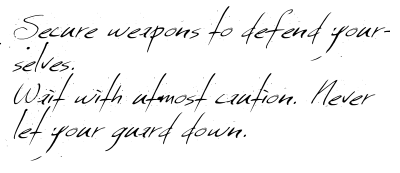
\includegraphics{OEBPS/Images/memo9.png}\\

Would that mean they would be faced with a fight? Would that fight be
with Security Bureau officials stationed at the Correctional Facility?
But there was no way Bureau officials would come all the way down to the
hygiene management room. The one man who had worked in this room had
been killed. He was already a corpse. No one would have business here.

He swallowed his saliva. Wait with utmost caution. Never let your guard
down. Inukashi pounced on the wall switch, and turned the lights off.

"Hey, what was that for? Now I can't see anything," Rikiga complained.

"That was bad."

"Bad? What was?"

"The lights. We turned the lights on."

"So what? When it's dark, we turn on the lights. Electric lamps might be
a luxury in the West Block, but here in No. 6 they're commonplace."

"Dumbass, that's not what I'm talking about!" Inukashi said testily.
"What are we gonna do if someone saw that light?"

Even in the darkness, he could see Rikiga's features tense. Inukashi's
eyes were naturally used to the dark. Damnit, we didn't even need these
lights in the first place.

"It'll be alright," Rikiga muttered. His voice was hoarse and hard to
hear, like he had forced it out of his throat. "No need to get so jumpy.
Stop acting like a lost rabbit. That light was on for maybe one, two
minutes max. Who the hell is going to care if the hygiene management
room burns down? You said it yourself: this place is like Paradise. It
doesn't even have surveillance cameras."

"It has been, up until now."

On one hand, Getsuyaku had been marked as a suspicious person, and had
been shot and killed. On the other, Nezumi and Shion had been able to
infiltrate the Correctional Facility successfully. This connection had
raised the question of whether the cleaning staff were on the same side
as the intruders, or whether they had collaborated together.

If that was so, was not this room more of a dangerous territory than a
Paradise? It was likely that surveillance had been tightened around the
area. It was very likely.

The black dog suddenly got to its feet. It cast its eyes around with a
low growl. Its gaze quickly trained on one point―the door. The door
connecting to the Correctional Facility. The black dog continued
growling at the metal door that only opened from the Facility side.

Shit.

Inukashi snatched a gun and hurled it at Rikiga. Rikiga barely caught
the outdated carbine in his hands. His lips trembled.

"Inukashi... what's going on? What's going to happen?"

"A visitor, old man. An unwanted one at that."

Thud. This time, there was a sound behind them. The entrance. He could
feel the moving presence of people through the worn grey door.

"A pincer attack. You must be kidding me." Shit, we've done it again.
We've made another mistake. A life-threatening one. Inukashi chewed his
lip. He knew it was useless. He could chew his lip to shreds and it
would undo none of the mistakes they had made.

Inukashi, get moving.

Nezumi's voice echoed in his ears.

A thousand regrets aren't going to open a path for you, but one act
will. Move. Just move.

Why do I hear his voice? Even at a time like this―no, maybe it's because
we're in this situation that I hear it.

Move. Search for the path to life.

Shut up, Nezumi. I've learned my own fair share of tricks to keep myself
alive.

He grasped the bag.

"This way."

He rammed his body into the door that led to the waste collection area.
The door did not budge. An alarm went off. The metal door was opening
up. He could see the tips of military boots.

"Inukashi, this." Rikiga touched the switch on the wall. The doors slid
sideways.

"Alright!" Inukashi roared to cheer himself on. The dogs swarmed into
the collection area behind Inukashi and Rikiga. Hamlet and Cravat wove
swiftly between their legs.

"Ugh, it smells." Rikiga broke into a coughing fit. He was right; there
was an odour. The stench of rotting meat juices filled the air. It was
no doubt the odour from the capsule that he had given Getsuyaku. The
capsule had been sucked in through a vacuum and brought to the
collection area along with other waste. If he had not been shot through
the chest, Getsuyaku would probably be sorting through this pile of
trash tomorrow. He would have been at his usual job.

"Makes me want to throw up," Rikiga groaned softly. A light flared
inside Inukashi's head. He swung around to see Security Bureau officials
with guns in hand beyond the glass. They had stormed into the small
room.

One, two, three, four... four people.

"Follow me, old man."

There was a small power shovel in a corner of the collection depot, near
the waste outlet. With this, Getsuyaku would deposit the waste onto the
conveyor belt and take it to the incinerator. Inukashi hid himself
behind the yellow-painted heavy machine.

The lights came on, illuminating everything with a glare.

Why do people from No. 6 hate darkness so much? Inukashi thought idly.
Why do they hate what they can't see, places light can't reach, and the
fact that darkness exists? Why do they try to illuminate it all?

Security Bureau officials opened the door and stepped in. Suddenly, they
covered their noses and mouths with their hands and bent over double.

"What is this?"

"It stinks."

All four of them retreated. All of their faces were contorted. One of
them fell to his knees and vomited on the spot. Inukashi grinned in
satisfaction, and still grinning, aimed his gun.

Hah, what kind of Security Bureau officials are these? They've got huge
egos but no balls to go along with them. I can't believe they're making
such a fuss over a little smell. Hmph, so that makes them softies as
well as crazies. Makes me laugh. You guys should all go home and suck on
your mommy's nipple.

He pulled the trigger.

An impact slammed into him. He felt like he had been hit hard in the
forehead. He tumbled backwards, and he felt a dull stinging from his
neck up.

"Horrible. What kind of aim have you got?" Rikiga shouted.

"Cut me some slack, it's my first time. Why don't you try shooting, old
man?"

"Never. I'm a pacifist through and through. I could never fire at other
humans, even if they're Bureau officials."

"I'd like to see you hit your target at least two, three times before
you make a sick joke like that."

The Security Bureau officials fled desperately from the stench. They
would probably not set foot into this place again without gas masks.

How fragile they were.

They were not civilians; they were specially trained Security Bureau
officials. Yet, they could not even endure a mild odour like this.

But at this point in time, Inukashi wanted to thank them rather than
scorn them for their fragility. The officials had bought them some time.
He was not foolish enough to be relieved, thinking that danger had
passed. But bought time was bought time. He could draw a breath.

But what'll I do with the time I bought?

After I catch my breath, what'll I do next?

He licked his bottom lip. His tongue ran across the dry membrane.

This room had only one entrance and exit: it was the door they had come
running through. The Security Bureau officials―their enemy―were
stationed outside. They were in a sealed room. There was no escape
route. Soon, those crazy softies are going to attack us. When that
happens―

The more he thought about it, the more hopeless the situation seemed to
him. But Inukashi did not give up. We'll manage. There's no way we'll
end like this. Isn't that right, Nezumi?

He didn't know whether he was believing in Nezumi or himself. But he
knew that he believed. He believed―so he did not give up.

We'll manage. We'll make do. We won't be finished off like this.

"Inukashi." Rikiga grabbed his shoulder. "What are they planning to do?"

"Huh?"

Inukashi glanced at the small room, and inhaled sharply. He stood rooted
to the spot.

The Security Bureau officials were loading in an odd-looking device. It
was about as big as the black dog growling fiercely at his feet. One end
of it fanned out widely, and the other end narrowed to about a third of
the width. Numerous spiralled tubes extended from it, but Inukashi could
not see where they led. The body, as well as inside the mouth of the
machine was a colour between grey and blue, and shone in the light. It
reminded him of a highly- polished brass instrument.

"What's that? A huge trumpet?" Rikiga's face relaxed comically, but his
voice was a mixture of tension and fear. "They should have told me there
was going to be a recital. I would have worn my dress coat."

Inukashi was too on-edge to respond to Rikiga's joke. He couldn't
swallow the breath caught in his throat. The thudding of his heart rang
in his ears so loudly, he felt like his eardrums would burst.

Various scenes in the West Block came back to him vividly. It was right
after the Hunt. His surroundings were an expanse of rubble.

The market, where throngs of people moved to and fro among the barracks,
tents, and two-storey brick houses that lined the street, was razed
completely. All had turned to debris.

This destruction did not come from blasting explosives. There had been
no distinctive smell of gunpowder. He had also not seen any burns or
singes. There had been no embers, nor rising smoke. No. 6 had not used
firearms as it usually did for this Hunt. He even felt like No. 6 had
used a giant hand to crush the whole market.

But what had No. 6 used instead of a giant hand?

"Acoustic shockwaves."

Rikiga's ear twitched."Wait, what did you just say?"

"No. 6 used acoustic shockwaves for the Hunt. Like spleen whales do, or
sperm whales, or whatever they're called."

"What are acoustic shockwaves? Where did the whales come from? Can you
explain it in a way I can understand?"

"I can't. I'm just repeating what Nezumi's told me. Old man, you saw for
yourself what happened to the marketplace."

"Yeah―it was a clean sweep. The perfect model of a cleanup. And you're
saying they used acoustic shockwaves for that?"

"Yeah."

Rikiga's eyes opened wide. They bulged so much, Inukashi could count
each capillary running along his eyeball.

"Inukashi, so you're saying that weird trumpet―"

"It might be a smaller version of what they used in the West Block."

Might be? Hey, Inukashi, you can't fool yourself anymore. That has to be
a miniature sound cannon. That's what No. 6 was developing.

"And―and they're going to fire that on us?" Rikiga bellowed.

"Don't ask me; ask them. They're the ones with the answers."

Rikiga growled still. Through the darkness, Inukashi could see his face
growing pale. Inukashi aimed his gun, and fired at the blue-grey weapon
of destruction before him. This time, he did not stagger. With great
effort, he held his ground and maintained his posture.

He could not discern where the bullet had hit. Perhaps it had not hit
anything. Perhaps it had flown away into the distance like a whimsical
crow.

"Couldn't you have attached an automatic target tracker?" he grumbled.

"Do you think the West Block would have such a luxury item?"

"Hah, I'm sure you pinched as many pennies as you could. Look what
you've ended up with: something slightly better than a toy."

"That's not the gun's fault. It's your aim."

They peeked out from behind the power shovel at the small room. The
Security Bureau officials were moving busily. They showed no signs of
retaliation. They did not fire a single shot back.

They don't need to. They did not need to hit a wretched man right before
delivering his execution. That was probably their concept.

How compassionate of them. Brings tears to my eyes.

"Inukashi, hey, Inukashi. What are we going to do? If we go on like
this, we'll be―" Rikiga yelled and ducked down. He cradled his head and
arranged himself in a defensive position. His whole body was shaking.

There's no way I'm gonna die here. I haven't been born into this world
to die in a place like this.

Violent emotions churned in his chest. He had never thought about why he
had come into this world. Not once. It had seemed so trivial, he had
never felt the need to think about it. To Inukashi, finding a reason for
being born was nothing more than a foolish game. He had been born into
this world, and that was why he was going to live in it. That was it.
His life was no one's but his own.

I'm going to decide whether I throw this life away or protect it. It's
no one else's business.

He fired wildly. Shooting skills? Go to hell. The glass dividing the
room and the collection area shattered with a mighty crash. The Bureau
officials' panic was apparent.

The stench had become a torrent, tiding into the small room.

Move! Nezumi's hand thumped his back. Move, Inukashi. Act in order to
live!

Just what I was planning to do, Inukashi answered in his head.

He sprinted up.

The black dog bounded past him and gave a great leap. It soared through
the broken window, making straight for the Bureau officials.

\hypertarget{index_split_037.htmlux5cux23calibre_pb_68}{}

\protect\hypertarget{index_split_067.html}{}{}

\hypertarget{index_split_067.htmlux5cux23calibre_pb_0}{}

\hypertarget{index_split_067.htmlux5cux23calibre_toc_4}{%
\subsection{CHAPTER 3}\label{index_split_067.htmlux5cux23calibre_toc_4}}

\subsubsection{Cease from the struggle of war's impartial contention}

\emph{"Zeus-sprung son of Laërtes, Odysseus of many devices,}

\emph{hold back, cease from the struggle of war's impartial contention,}

\emph{lest wide-thundering Zeus son of Kronos be angry against you."}

\emph{-Homer, The Odyssey}

The door of the elevator was open by a crack. Nezumi hooked his hand on
it.

Give me strength. Please. He prayed, but not to God. He prayed to the
girl with the wilful gaze. Safu, give us strength. A little more, just a
little strength for us...

The door opened, but not by enough. They could not escape yet. Nezumi
heard laboured breathing behind him.

"Shion..."

Shion was getting to his feet. He silently stretched his hands out, and
his fingers grasped the door. They looked at each other. Tsukiyo poked
his face out of the folds of superfibre and cried once, loudly.

Cheep!

Nezumi and Shion took that as their signal to push the door with all
their might. The gap widened so that one person could slip through with
some effort.

The elevator careened. His feet stumbled unsteadily.

"Hurry, get out!" Nezumi pushed Shion out before squeezing through the
gap. The elevator gave an irritating screech, which turned into a
rumble. It hurtled downwards as if it had been waiting for the two to
escape before setting off.

Nezumi closed his eyes for a moment. My gratitude, Safu. Sweat poured
down his cheeks. The wound on his leg throbbed. His heart pounded
against his pectoral muscles from the inside.

He was in pain.

His mental and physical strength was whittled down, crumbling off, and
barely remaining. He was in pain, yet―this pain, this throbbing, this
heartbeat was nothing less than proof that he was alive. He was still
alive. Still alive.

He opened his eyes and took in his surroundings.

He saw scattered glass shards and a wet corridor. Two men lying dead.
The black-haired soldier and Rashi were unchanged from how Nezumi and
Shion had left them.

One was lying in the corridor covered in blood, and another was thrown
out on the ground near the wall. The barriers were gone. The sprinklers
were off. There was no human shadow or presence.

Nothing. Only Nezumi and Shion's breathing could be heard, almost too
loudly.

Whoom. Something exploded. He spun around and saw smoke coming out of a
room at the end of the hall. It was the room they had fallen into after
destroying the ventilation duct. Flames soon licked through the door
left ajar.

It was burning.

A similar-sounding explosion rocked them from the floor below. He could
hear the commotion and people screaming.

The computer systems on each floor were executing the same program of
exploding and bursting into flames. Like loyal subjects, all devices
within the Correctional Facility were following after the mother
computer.

Were these machines following in their master's footsteps, despite the
fact that they had no soul? No; they had only been programmed to do so.
The mother's failure meant death for all systems within the Correctional
Facility. They were configured to self-detonate as soon as they stopped
receiving signals from the mother. It was nothing as lax as the
information being wiped or deleted, or the device itself going out of
operation. They were forcibly destroyed.

So were they following the master to her grave after all? It was forced
suicide. The system ended everything along with itself. It allowed
nothing to survive. Had the creator of this system directly applied the
dictator's logic?

The flames had crawled into the corridor. The heat attacked them. Smoke
filled the air thickly. None of the extinguishing devices were
operating. Neither smoke extraction devices nor air filtration devices
were working. A system which had been so flawlessly tuned to eradicate
unwanted objects was completely useless.

"Shion, go down. We have to escape downwards."

They clambered down the stairs. Hot air blew at them here as well.
Personnel were screaming and rushing to escape.

"Fire! It's a fire!"

"No, it was an explosion! Suddenly I couldn't control the thing anymore.
Oh, look at this mess!"

"Help me! My arm, it's been blown off―a doctor―"

"Oh, I'm so scared―we have to escape, quickly!"

"What's going on? What's the matter? Nothing seems to work. The
automatic doors aren't opening. What's wrong with the lights?"

"Someone, this person's covered in blood. Someone, please!"

"The smoke... it's choking me."

"We can't use the elevator. The stairs―only the stairs are left."

It was truly a pandemonium. A mob of lab coats stormed the stairs as
each one tried to get down before the other. Some slipped and fell on
top of others. Some tried to help their friends; others stepped over the
fallen ones and fled; some wept; some cried out directions for the
emergency route. A woman helped a bleeding man to his feet; a man shoved
a staggering woman out of his way as he ran past her―each one showed his
true colours in this tragic scene.

An even louder explosion shook the air.

It had evidently blown a hole somewhere, for the air began to move in a
current. The smoke cleared somewhat. If even for a moment, they could
catch their breath.

Again, the same sound, and the faint roar of a crowd.

Nezumi turned around and confirmed that it had come from the direction
of the prison wing. The trapped prisoners were causing a commotion. But
if all of the prisoners' wing had been computer-monitored, then every
door should be unlocked by now. Perhaps that noise was the sound of the
prisoners cheering and roaring at being set free.

But if that was so...

They reached the third floor. The flames, smoke, and confusion were more
subdued than the fourth. Some people had caught a breath on the
stairwell, restored their reason and were attempting to escape this hell
by supporting each other.

Can we keep at it and escape? Hope flared. A ray of light pierced the
darkness.

All systems had died. The Correctional Facility was being reduced to a
mere building, an empty shell with no function. With the addition of the
prisoners, the chaos was bound to get worse.

And when that happens.... Perhaps it would be easy to take advantage of
this situation to escape. There was not much blocking their way.

"Shion, let's go." Nezumi restrained his over-eager heart, and grabbed
Shion's wrist. Shion did not move. "Shion!" he said urgently. "What is
it? We have to get out of here."

"Why did you kill her?" Shion muttered, barely moving his lips. It
sounded almost like a gasp. Nezumi let his hand go, and met Shion's
gaze. He could feel his blood turning cold. He was freezing over
gradually from his extremities.

"Nezumi, answer me. Why did you kill Safu?" Shion's voice caught in his
throat, and took on an unnatural murky tone. Nezumi felt like he was
listening to static-filled music through outdated speakers.

"We― I came here to save Safu. Save her... not kill her." Shion's whole
body began to tremble, but no emotion could be read from his face. Not
agitation, nor wrath, nor sadness, nor anguish.

"Shion, we were too late. She was already―"

"Safu was alive." Shion's murky voice jolted him sharply. He felt like
he had been slapped on the cheek. "She was living, and standing right in
front of me."

"That was an illusion. You should have known yourself. That wasn't her.
It was just an illusion."

"No! No! No!" Shion yelled. "Safu was alive. She was alive, and that was
why she could appear in front of me. Nezumi, I don't care what form she
took. Safu was definitely alive."

"...No matter what form, huh."

"Yeah. Safu may have lost her body, but she was alive. She was alive and
waiting for me. I needed to save her. I should have stayed here with
her. Isn't that right, Nezumi?"

Safu was alive. Was she? Had she really been? Nezumi ground his teeth.
She had been alive and waiting for Shion. She had been waiting
devotedly, just for him. She had been alive just to see Shion once
again. And her wish had been granted.

Safu, Shion overcame hardship and danger to come to you. You were able
to meet your most beloved person. But what you wished for next was to
disappear from Shion's sight. Yes, you wished for it.

You didn't want Shion to see you.

That was why...

"Shion, we couldn't have saved her. She and the mother were fused
together. And she... she chose to die with it."

"Is that your reason? Your reason for murdering Safu?"

"Then what should I have done?" Nezumi yelled. His blood, which was
supposed to be frozen, boiled and raced through his body in a hot
stream. "Don't you understand how she felt? She summoned us because she
wanted to see you. And―and couldn't you see it was because she wanted to
be saved? I don't mean escaping from the Correctional Facility. She'd
already known it was impossible. That was why she wanted you at least to
save her from that wretched situation. You were the last person whom she
wanted to see her like that. I mean, wouldn't you feel the same? You
understand, right?"

Nezumi's breathing was erratic. Shion's expression did not change. Not
even a twitch of an eyebrow. The smoke stung at Nezumi's eyes.

We have to run. We can't waste any more time here. His thoughts were
clear, but his feet would not move. They quaked at Shion's eyes.

"Shion, I can't think of it as you do. We were too late. Safu was
already dead." They were his true thoughts. "You aren't looking at
reality. It would have been impossible to separate her from the mother.
She even said so herself: she had no body, but she was still trapped.
She said it hurt, that she wanted you to set her free. She wished to be
set free from that situation, from her humiliation."

He was not wrong. Shion was the one with the wrong idea. He was unable
to accept the reality of losing Safu. He was trying to avert his eyes
from the truth.

"You used her." A low, low mutter. Nezumi did not catch it.

"What?"

"You used Safu to destroy the mother. Isn't that right?" Shion's eyes
shifted slowly from right to left. Tsukiyo peeked out from the
superfibre, but soon ducked back inside again.

"Destroying the Correctional Facility was your purpose from the very
beginning. Your object was never to save Safu, it was to destroy the
Correctional Facility, and to use it as a gateway to destroy No. 6. You
were waiting for that chance all along. That was why you didn't hesitate
to destroy the mother. You didn't hesitate at all. You used her for your
own purposes. You sacrificed her."

Nezumi stared at Shion. Used her? Didn't hesitate at all? Sacrificed
her? Shion, you really think so?

But is he wrong?

He heard a voice questioning him back. It was not Shion's. It was his
own voice. Did you not use her? Did you not sacrifice her? Did you not
prioritize your own wishes over saving another life?

Didn't you? Didn't you? Didn't you?

Roar. Roar.

A knot of people wearing dark green shirts came storming down the
stairs, screaming. They were prisoners. Their loud cheering hit the
walls around them, bounced, and echoed clamorously.

Roar. Roar. Get out, get out.

"Stop! I said stop!" The Security Bureau official's orders were drowned
out by the din. Suddenly, a gunshot rang out. A man trying to run past
Nezumi careened backwards and fell onto the floor in the corridor. He
had been shot through the head.

"Stop! Stop, or I will shoot!"

"Run! Get outta here!" the prisoners yelled. "Don't stop! Escape! Hurry,
hurry and get outta here!"

All the prisoners had bloodshot eyes. Some were foaming at the mouth.
Every one of them roared like beasts as they ran.

To become a prisoner of the Correctional Facility meant death. Whether
guilty or not, regardless of the severity of the crime, as soon as they
were imprisoned, they were on death row.

We're going to get killed anyway, so why not cling to this miracle?
We'll latch onto this one-in-a-million chance, and be free.

To the outside world. To the outside world. Run to the light.

Gunshots. Sprays of blood. A white-haired prisoner crumpled over the
railing. Gunshots, explosions, smoke, fire.

"Shion, it's dangerous here." Nezumi grabbed Shion's arm and yanked. He
met no resistance. Shion staggered and bumped his shoulder on the wall.
He slid to the ground, still leaning on the wall.

"Nezumi... I'm sorry." A whimper spilled from his bloodless lips. "I'm
sorry. I―I―" Shion covered his face with his hands, and drew several
ragged breaths.

"I know," Shion said. "I know we had no choice but to do it. You granted
Safu's wish... I have no reason nor right to blame you. It was me... I
should have been the one to do it. It was my job to set Safu free. But I
couldn't. I was scared... and I couldn't do it. I leaned on you again,
thrust everything onto you, and made you do the dirty work. I didn't
want to acknowledge my cowardice, so I blamed you, ran you to the
ground..."

Nezumi looked down at Shion's snowy hair. Despite having been through
such a hellish ordeal, it had not lost any of its lustre. Every single
hair shimmered elegantly.

"I got you involved, and even dragged Rikiga-san and Inukashi into it...
and if the result was this.... Nezumi, we didn't come here for
destruction. We came here to give salvation. But look―"

"We came for destruction."

Shion lifted his face. It was smeared with sweat and blood.

"You're right. I had only one purpose, and it was to destroy the
Correctional Facility. I never had plans to save Safu from the
beginning."

"Nezumi..."

Nezumi looked away from Shion. He couldn't hold the other boy's gaze.

"I needed you. I knew that without your memory and judgment skills, it
would be impossible to get around inside the Facility. You were my last,
and my best trump card. I thought for a long time how I would use you,
and... this is the answer. The thing about Safu was just an excuse. I
just... used you and her to satisfy my own purposes."

Yes, Shion, you aren't wrong. I betrayed you. I was tricking you all
along. You didn't get me involved; it was the other way around. I set
the cunning trap.

"My plan was a success. Look at this confusion. The Correctional
Facility is crumbling. Shion, I―I directed things to proceed according
to my intentions. Frankly, I didn't expect it to turn out so well. You
served your purpose a hundred times better than I expected. You were...
really useful to me."

Shion stood up unsteadily.

"Nezumi, what are you talking about?"

"I never believed that Safu would be safe. The moment she was
imprisoned, I knew the possibility of her escape was close to nil.
Shion― saving Safu never mattered to me. When I planted the bomb in the
mother, I was only thinking of destroying it and getting out of there as
soon as possible. That was it."

The superfibre cloth slid from his neck and fell at his feet. Had he
been bowing his head unwittingly? Nezumi stooped to pick the fabric up,
and stared intently at the boy in front of him.

"I'm not asking you to forgive me. It's not something I can apologize
for and be done with."

"What are you talking about?" Shion said loudly. "I'm not getting a
single word."

Really? Can you really not understand?

You're a liar, Shion. You do get it. You understand every single word.
And you'll never forgive me. You'll lose faith in me and loathe me. Or
would you―

Cheep!

Tsukiyo squeaked sharply. Nezumi felt his spine tense. He felt like
transparent arrows were stabbing into him. It was murderous intent.

He turned around. A man stood there, aiming a gun at him. He was not a
Security Bureau official. He was one of the soldiers who had been under
Rashi's command.

Nezumi had noticed him too late.

"Shion, duck!" He shoved Shion as hard as he could. Immediately, the
impact came. A beam of light seemed to pierce his entire body.

It scorched him.

He tried to scream.

Escape, Shion. Hurry, he thought, but no voice came out. Somewhere―
somewhere in his body, he was burning. It was hot.

"Nezumi!"

He could see Shion, wide-eyed. He could see clearly the boy's screaming
mouth, his extended hand, and the shape of his fingers. The image was so
vivid, it seemed hardly real.

The vivid scene blurred, and darkness closed in.

All colour faded.

* * *

Raugh!

The black dog was thrown out across the floor. Its limbs convulsed as it
foamed at the mouth. The Bureau official had propped himself up and was
holding a small gun in his hand. The black dog eventually stopped
moving. Despite its aggressive nature, it had loved to nap in the sun.
It would often lie in the sunlight much like it was doing now,
stretching its legs out. It had a temperamental disposition, but it was
loyal to Inukashi,

I'm sorry.

Inukashi cast a glance over the dog, and apologized inside his heart.
I'm sorry for putting you through this. Forgive me.

He could see down the barrel of the gun. He could see the hollowed
cheeks of the thin-faced man who held it. Inukashi did not flinch. He
did not stop. A moment of hesitation, a moment of confusion could cost
him his life. Once he started to move, he had to keep moving. With the
enemy before him, he had no option to cower.

He aimed his gun and fired blindly in furious succession.

Damnit, damnit, you bastards. You arrogant murderers. You're all cruel,
dirty thieves. Give back everything you've stolen from us. You guys have
trampled over everyone in the West Block for this whole time. You killed
people indiscriminately. You cold-blooded murderers. Have some shame.
That's right. You shameful, despicable people. Damnit.

He mentally hurled as many insults at them as he could. He could not
voice his vilification. If only his wrath could turn into bullets and
shatter that blue-grey weapon.

Can't you give us a miracle like that for once, God? You were quick to
turn your back on the West Block, like a mother abandoning her infant on
the barren plains. Doesn't your moral conscience bother you at all? So
give me a miracle, at least, to make up for it. Hand over that miracle
so we can survive.

His foot slipped. He lost his balance and landed on his bottom. Bullets
bounced at his feet. If he had not fallen, he would have been shot
cleanly through.

Phew, I still have some luck left.

"Don't move, filthy sewer rats." Bureau officials pointed guns at them.
Simultaneously, a nerve-racking bass rumbled.

"We'll exterminate you well. Be prepared."

Sewer rats? Don't you dare put me on the same level as those lowly
animals.

Inukashi tried to pull the trigger, but realized the gun was out of
bullets. He glanced at the power shovel.

What the hell are you doing behind there, old man? The baritone rumble
was issuing from the somewhat comically wide mouth of the shockwave
cannon. Preparations seemed to be set.

What? No way. Is this it? A frigid wind blew up at him. Is this the end?
Am I gonna die here? That can't happen. You gotta be kidding me. Nezumi,
this isn't what you promised. The whole show is gonna be ruined before
the main actors even appear. What the hell do I do now? Do something, do
anything, Nezumi!

Suddenly, the lights went out. An alarm sounded.

"What? What is it?"

"I don't know. Something's happened inside."

"Hey! Did you hear an explosion?"

"Huh? Oh, now that you mention it―"

Inukashi could feel strongly the agitation of the officials.

"I can't see! I can't see anything in here!"

Shrill screams, almost shrieks, echoed in the darkness. It's the same as
with the smell. They're really, really weak. Inukashi smirked.

The people of No. 6 were so unbelievably, so laughably weak when even a
small change occurred in their clean and comfortable environment.
Perhaps soldiers would have had a little more resistance. But the
Security Bureau officials were cowering, clearly exposing their
fragility.

Look at what a loss you're all at. You build that murder weapon with a
cool face, but you're afraid of the dark. Disgusting. Inukashi hurled
abuse at them, still sitting on his bottom. He restrained himself from
rushing out.

"Not yet. Don't rush it," he told himself.

The alarm grew louder. Its enormous volume rattled his eardrums.

Emergency alert. Emergency alert.

Level 5, Level 5.

Emergency evacuation. Emergency evacuation.

All personnel, evacuate immediately.

Level 5, Level 5.

"Level 5!? What is it, what's going on?"

"I don't know, but we should evacuate. We have to get out of here, or
we'll be in danger."

"Hey, there it is again. I heard it. Things are exploding everywhere.
Get out!"

"I-I wish I could, but it's so dark... why aren't the backup lights
coming on?"

"This is a trash depot. Do you think they have backup lights?"

Now! Inukashi leapt to his feet, using his whole body for leverage. I'm
used to the dark. You'll see how different I am from all of you.

"Bastards!" He yelled as swung his gun around. It hit something. The
dogs snarled and pounced. Inukashi started yanking out all the pipes and
cables attached to the cannon.

Bastards. Bastards. Making crap like this. You guys made a monster
that's good for nothing but killing people.

Level 5, Level 5.

Emergency evacuation. Emergency evacuation.

"Outside! Get outside! It's dangerous in here!"

"Yeah, get out! We have to evacuate!"

The Security Bureau officials fled through the door leading outside.

Inukashi stood, breathing heavily. Sweat poured off his whole body. But
he was shaking. He could not stop. His teeth chattered. His heart was
palpitating so badly, he had trouble catching his breath.

He fell to his knees as the strength left him. His dogs approached. One
with a patched coat pushed its nose up against him. Inukashi latched on
to its furry collar and buried his face in its soft fur. It smelled like
dog. He had known this scent for as long as he could remember. It was
the scent of his mother, his siblings, and his friends. It smelled more
sweetly than any flower.

Tears spilled over. They streamed down one after another. We're saved.
We've been saved. The dog licked away the tears on his cheeks. It's
warm. Oh, it's so warm. I'm still alive.

"I owe it to you guys. Thank you. Thanks so much."

"Inukashi..." Rikiga came crawling out through the door of the waste
collection area. "Looks like they ran off."

"Yeesh, old man," he gave a purposely long sigh. "What good are you
gonna be now? Were you off shopping for today's dinner or something?"

He gently brushed his tears away so Rikiga wouldn't see them. Rikiga
shrugged, and laughed softly in the dark.

"I told you, I'm a philanthropist. I'm also a born and bred gentleman.
No one is more ill-suited for killing than me. Fortune could turn every
which way, but I would never be able to go wild and let loose like you."

"Well, you can turn right back around and never come back again. You're
just a useless drunkard even when you're around, anyway. You'd only hold
me up."

"Nothing to be angry about," Rikiga said lightly. "Ah, but I have to say
that was an impressive fight. I have a new regard for you now. If I were
a girl, I'd have fallen for you right there. Bravo, bravo."

Inukashi wrinkled his nose at Rikiga's applause.

"You falling for me, old man? What a horror story. You just gave me the
goosebumps. I just came out of deadly territory, alright? I'd appreciate
it if you could lay off that stuff, it's bad for my heart. The last
thing I wanna do is keel over from fright here."

Rikiga paid no attention to Inukashi's insults. He cupped his hand
around his ear and listened intently. The alarm stopped as abruptly as
it had started.

Inukashi also pricked his ears.

He could hear something like the distant rumble of the sea, or distant
thunder.

What is it? What is that sound?

"Something's exploding inside the Correctional Facility," Rikiga said in
a queerly languid voice. "And that's not it... I can hear screaming in
there, too. It's in there. Yeah, I can hear it."

The door connecting the Correctional Facility to the waste processing
area was still open, which was why they could hear what was going on
inside. Two spaces which had always been firmly divided were now
connected.

"Hey, Inukashi. Is this a precursor? Is this the beginning?" His voice
quavered as it tapered off. Inukashi could not see his face, but he knew
that Rikiga was probably flushed with excitement. He did not even need
to look. My face is probably that colour, too, Inukashi thought. I'm
excited. I'm restless.

It's beginning. It's finally beginning. It's actually beginning.

Nezumi, Shion, you guys actually did it. I don't know what the hell you
did, but you did it. You set the alarms off throughout the Correctional
Facility. Level 5. Is that the highest hazard level? If it was... hah,
this is getting interesting. This is gonna be fun.

Those must be gun salutes in the distance.

Inukashi had been licking his lips unwittingly.

Nezumi, that fraudulent bastard wasn't just a talker. He did what he
promised.

"You think the Correctional Facility's going to come tumbling down?"
Rikiga murmured, his voice still trembling.

Suddenly, the lights flashed. They went out again, and the room sank
into darkness. The door closed, opened, tried to close again, but
stopped at about two-thirds of the way.

"What is it? Is it practicing a dance?" Rikiga cracked a lame joke.
Inukashi didn't even feel like laughing.

"Go dance along with it, old man." He was licking his lips again. This
isn't a dance. These are its last spasms. Its last struggles before its
life gives out. Just like that black dog, the Correctional Facility is
writhing in pain at the brink of death.

"Don't tell me the whole building is going to collapse." The excitement
faded from Rikiga's voice, and uncertainty crept in.

"All's good and well if it collapses," Inukashi replied. "Once this
place becomes a mountain of rubble, I'll be the first to plant a
memorial tree." I'll plant one for Getsuyaku, my black dog, and the
countless people who were murdered here. A tree that'll grow huge and
bloom with pure white flowers.

"You sounded so happy the other day wishing this place would come
falling down, old man," he added.

"That was a form of expression. I don't mind the Correctional Facility
falling down, but I have a bit of a problem with this building becoming
a pile of rubble."~

"Why?"

"Inukashi, think really hard about it. If this building collapses
completely, the gold bullion underground will be buried along with it.
It's going to be a hell of a lot of work digging it back up."

Inukashi stared at Rikiga. The man's face was earnest.

"Old man... did you really believe that?"

"What?"

"The story about the gold bullion. Do you actually believe it's down
there?"

Rikiga's eyes wandered. His throat contracted.

"Inukashi, what are you joking about now? Of course it's there. My
information sources are trustworthy. There's no room for doubt."

"Okay, if you say so," Inukashi said indifferently. "Who was your source
again? Ann or Oon or something like that, right?"

"Sulu, the redheaded beauty. She heard it directly from a high official
of No. 6, in bed. No doubt about it. This tip isn't a dud."

"Is that how it goes?"

"Yeah. You might not know, since you're still a snot-nosed kid and all
you deal with are dogs. The thing about men is that they can't lie to
women after the deed. Wives are a different story, but men don't lie to
women they buy. They don't need to."

"That's why they accidentally spill the beans about confidential stuff
they'd never talk about."

"That's right. So you do understand."

"And can you trust this Sulu woman?"

"I sure can. I pressed her over and over about whether this story was
true. Sulu said she definitely heard it. She's sure of it, and so am I."

"Are you two together, old man?"

"None of your business, kid. Inappropriate subject matter for children.
As a well-meaning adult, I refuse to answer. No comment."

"Anything that comes out of your mouth is inappropriate, old man,"
Inukashi retorted. "Any well-meaning intentions of yours are probably
dissolved in alcohol by now. You're as inappropriate as adults get. I
would never want my baby around you."

"Back to the topic," Rikiga said impatiently. "How does my relationship
with Sulu have anything to do with what we're talking about?"

"To get straight to the point, I'll just say that between you and
Nezumi, Nezumi would get girls a lot more easily. Yeah, I think
ninety-nine out of a hundred... no, all hundred girls would rather sleep
with Nezumi than you. Of course. And I don't think Sulu is an
exception."

Rikiga's brows furrowed theatrically.

"Inukashi, what are you trying to say? Stop trying to beat around the
bush. Do me a favour and be clearer about it."

"Clearer, huh. Well, there's not much to say, anyway. Say I'm Sulu, and
I love to watch plays, and I get totally hooked onto this good-looking
actor called Eve. If he whispered into my ear with that sultry voice of
his, what would I do? I think I'd be pretty eager to feed false
information to a certain beer-bellied old man, no matter if he was my
ex-boyfriend or not. Just a thought," Inukashi said offhandedly.

Rikiga swallowed hard. He opened his mouth and started panting like a
dog in scorching heat.

"How―no, how―why would Eve ask Sulu to do that? Th―there's no plausible
reason―"

"To manipulate you, old man. Actually, maybe I was part of the plan,
too. He wanted to draw us in by hinting to us about some gold bullion.
It's the easiest and most effective way. Doesn't it sound like something
he'd think of? He's unbeatable when it comes to being wily. He's
astonishingly smart. I'm actually really impressed."

Rikiga stood still and speechless for a good while.

"Inukashi... when did you realize that?"

"When? I dunno. I think from the moment I heard you got the tip from a
pretty girl, Nezumi was in the back of my mind. Hah, I guess that means
I know a little bit more than you about Nezumi's true identity, huh? Not
much to brag about, though."

"If you knew, why did you still come? Why are you putting your life in
danger to do this?"

"Because there's gold bullion."

"Huh?"

"I actually don't know why I'm not curled up quietly in my nest right
now. I really don't know. It's just―something I thought would never
break is breaking. Something I thought would never change is gonna be
turned upside down. It's almost as amazing as a mountain of gold. And
God's not making that miracle―humans are. An airheaded boy and the fraud
of the century. Doesn't it give you a thrill? It gave me a thrill.
That's why I decided to act on my own. I wasn't gonna wait 'til someone
changed things. I'm gonna go ahead and do it. I wanna think that I have
a role in changing the world. Nezumi and Shion threw that opportunity
down right in front of me. They said, 'How long do you plan on curling
up there and pretending you don't notice?' and tossed the bait in front
of me. Bait that's bigger than gold."

"And you latched onto it knowing you were being tricked."

"I guess you can say that."

"I see... so you got in on it and tricked me, too. What a shameful day
for Almighty Mr. Rikiga. I've been strung along by a couple of brats.
I've grown old. I think it's really hitting home now that my life is
entering its retirement stage."

"Hey man, don't be so down about it. It's just my guess. I think it's
about ninety-percent right, though. There's always the possibility that
Sulu seriously had the hots for you, and she gave you the gift of juicy
information."

"Serious about me, huh... impossible." Rikiga gave a great sigh, and
slumped his shoulders. True to his word, he suddenly looked like he had
aged by many years. "So what do you plan to do now?" he looked up at
Inukashi, and exhaled again.

"Me? I'm gonna wait."

"For Eve and Shion?"

"Yeah. Nezumi told me to wait here. What other choice do I have?"

"Like a loyal dog waiting for its master."

"More like a cunning fox preying on a field mouse."

"Where are they coming back from? From that half-open door?"

"Who knows? I can't read that far into it. I don't think even Nezumi
would know. They're gambling for all or nothing―there's no way they can
foresee that far. Climaxes are best left in the dark, anyway. So what
are you gonna do, old man?"

Rikiga sighed yet another time. His back was hunched and his posture was
truly that of an old man, though Inukashi wasn't sure if he was doing it
on purpose.

"I'll wait," he replied. "Feeling like a loyal dog."

"Even if the gold bullion was a lie?" Inukashi was a little surprised.
He had been almost certain that Rikiga would beeline right out of this
room as soon as he found out that the gold bullion was an illusion.

Here, you don't know what's gonna happen next. There's no way of
guessing what kind of danger is coming, and when it'll come.

Anyone with some smarts would get the hell outta here and go back home.
And Rikiga's not stupid. He might be prone to wandering off, blinded by
greed, but he's got the smarts it takes to survive. If not, he wouldn't
be able to hoard money in a place like the West Block.

Rikiga only got involved in things that benefited him. Emotions and
sense of duty were not in his criteria for taking action―only potential
wealth was. This was Rikiga's philosophy of life, and Inukashi agreed
with it. That was why he was taken by surprise.

"Why're you gonna wait, old man?" he questioned sincerely. He was truly
curious.

"Because I can't move."

"Can't move? Doesn't look like you're hurt to me."

"I'm out of breath, and my heart is palpitating. My legs and back are
shot. I have no choice but to rest here. Besides, there's nothing to
prove that you're a hundred percent right. Sulu's tip might be a good
one after all."

"You're saying Mr. Gold Bullion is just sitting on his ass under our
feet."

"Yeah. I've come this far believing in it. There's no way I'm going to
leave with nothing. If it comes to this, I'll clean out the Correctional
Facility of anything that's worth money. And I'll get you and Eve to
help. For free. I'm not taking complaints."

Inukashi shrugged, and turned aside. He wasn't convinced that Rikiga was
telling the truth. What was he waiting for? What was he staying behind
for? Inukashi was sure even Rikiga himself did not know the answer. He
knew at least that it was probably not because of his palpitating heart,
his shortness of breath, or the gold bullion, which was nothing but an
illusion.

So whaddaya know, the old man actually believes that they're coming
back. Inukashi meant to sneer, but ended up compressing his lips.

Changes are happening inside the Correctional Facility. It's almost
time. They're almost coming back.

In the dark, Inukashi quietly balled his hand into a fist.

* * *

"It's delicious," Renka sighed. "I didn't know hot tea could taste so
nice."

"More sugar? They say sweet tea soothes you when you're tired." Karan
placed the pot of sugar in front of Renka. It was something she had
bought to celebrate the opening of her store. It was a small and cheap
pot, but it was Karan's favourite.

Renka pinched her tear ducts.

"Karan―thank you. I'm so glad you're here. Thank you."

"Oh, Renka, don't cry." Karan placed a hand on Renka's knee, and added
strength to her tone. "You have Lili. Don't cry. Be strong."

Lili, who had been looking up at her mother with concern, gripped the
cup in her hands tightly. Karan knew how harsh it was to reprimand Renka
and tell her to be strong when she was so overwhelmed with uncertainty
and exhaustion. "Be strong"; "smarten up"; "try your hardest"―at times,
words of encouragement from others hurt the soul much more brutally than
insults.

I'm at my limit. What am I supposed to try harder at?

Karan herself had come close to screaming so. How ruthless, how shallow,
how crude they were―such superficial words of encouragement or reproach.
I know. But I have to say them.

"Renka, you have Lili and the baby in your womb. You're a mother―you
have to be strong. You could cry any other time. But now isn't the time
to let your feelings go, is it? You have to pull yourself together."

Renka blinked, and swallowed her breath. Then, she straightened her
back.

"Yes, senpai.{[}1{]}"

"As long as you understand. Be careful next time."

"Of course."

Lili's gaze darted between her mother and Karan.

"Ma'am, you're Mommy's senpai?"

Renka gently drew her daughter's shoulder close. "Yes, she is. My senpai
in life. I'd want her to teach me a lot more things in the future."

"Ma'am, you must be really old."

Karan and Renka looked at each other, and burst out laughing almost
simultaneously.

"How mean of you, Lili," Karan exclaimed. "That's not true. Your mommy
and I are only―oh, we're eight years apart. I guess I am pretty old."

"Oh, Karan!" Renka laughed, and softly brushed the tears from her eyes.
"No, Karan, I really am thankful. Who knows what would have happened if
I was alone. I would probably be bawling from anxiety."

"You're not that weak," Karan said firmly. "You would have gotten your
strength back as a mother without me telling you to. And―you know,
Renka, this might seem like a temporary fix, but why don't we wait a
little longer for Getsuyaku-san? I feel like it's too soon to give up
hope."

Perhaps it was really just a temporary fix, something to disguise the
truth. But sometimes, you needed that something to ease your conscience,
something to mask the grim truth. Like a spoonful of sugar in a cup of
tea.

Renka put her cup down, and nodded slowly.

"Yes, yes... you're right. It's too soon to give up hope... absolutely
right. I'll wait for him a little longer. Maybe he'll come home
tomorrow."

"Right." Karan almost sighed. As long as Renka could not confirm
Getsuyaku's safety, she would have to keep waiting for her husband, and
Lili for her father.

It was too soon to lose hope. Yet hope without direction was a painful
thing.

Karan felt Renka clasp her hand. Renka's fingers were warm and soft.

"Karan, I won't be defeated. Even if by some chance, he
doesn't―Getsuyaku doesn't come home... the two of us will live―no, the
three of us will live together. I'm going to give birth to Getsuyaku's
child. I'll have his baby, and I'll raise it proper."

Strength shone in Renka's gaze. No hint of her previous tears remained.

"I have people like you who support me, so I'll be alright. I'll do what
I have to do. I'm a mother, after all."

"Renka!" Karan circled her arms around Renka's slender neck. "You're an
incredible mother. The best."

Look at us, Fate. Look how strong we can be. We won't be swallowed up.
We'll hold our ground and keep on living. O Fate, No. 6, we won't
submit; we won't be trampled on.

"Karan, there's one other person I'm actually concerned about." Renka's
tone turned heavy.

"Yoming, isn't it?"

"Yes, it's my brother... I'm wondering what he's trying to do. I just
have this nagging feeling that―has he come here?"

"Yes, he has."

"What was he like?"

"Well, let me see... he seemed to be worked up."

They heard a scream. It was from outside; it came from the direction of
the front entrance. It was followed by what sounded like someone falling
down. Karan stood up and hastened to the door. She peered through the
blinds. A group of men were squatting under a street lamp. A chubby
woman was cradling one of the men in her arms. Karan remembered her. Her
name was Koka, and she ran a tavern. The young man in her arms looked
like her second son. He was a boisterous youth and a spitting image of
his mother, and was dedicated to his job at the tavern and helping his
mother out. Once in a while, he dropped by Karan's shop. Last time, he
had bought all the butter rolls on the shelf, laughing and saying it was
because his mother adored them. Karan did not know his real name, but
she remembered hearing him being called "Good Guy Appa".

Half of Appa's face was covered in blood, and he was slumped against his
mother's arm with his eyes closed. He did not stir. He did not seem to
be breathing.

Karan burst out into the street.

"Koka, what's the matter?"

"Oh, Karan! My son―they got my son."

"Who did it?"

One of the men swung his fist in the air. "The army. The army shot at us
with guns."

Karan felt a jolt as if she had been hit by lightning. She thought for a
minute that she had been the one to collapse noisily on the road. But in
reality, she had clasped her hands tightly together, willed her legs to
stand fast, and was holding her ground.

I knew it. I knew it. I knew it.

"Army? What are you talking about? There's no such thing as an army!"
Koka wailed through her tears.

"There wasn't supposed to be, but there was. They weren't dressed like
Security Bureau officials. They were in military gear. And―and those
guys, they... they started firing at us..."

"Wait!" Karan said sharply. "Give me more details. You went to city
hall, didn't you?"

"Yeah. There was a summons through the Internet. We were on the move
because of it."

"A summons..."

"It was about this scary, mysterious illness. All these citizens are
dying, and yet the authorities aren't doing anything. And get this―the
mayor and all the big-shots have vaccinated themselves already, and plan
to abandon the rest of us. How could we let that pass? That's why we
stormed the Moondrop. You should have seen the amount of people there.
It looked like they came out from all over the city. Even Chronos
residents. We formed one huge mob and headed for the Moondrop. Our plan
was to get inside and see the mayor. That's what the message told us to
do. It told us to protect our own lives, and get our hands on that
vaccine. And that wasn't the only thing."

The man swallowed, and shook his fist even more furiously.

"We've been mistreated all this time. Our living conditions aren't even
half as good―no, even a tenth as good―as people living in Chronos. Even
though we're the same citizens. All this time we'd given up, thinking it
couldn't be helped. We all thought we had no choice but to bear with it.
But I've had enough of that. A horrible disease is going around right
now; I'm not gonna be left behind with no means of dealing with it."

Another man got to his feet. Blood soaked through the cloth wrapped
around his forehead.

"Yeah, that's right! Some consideration they must have for us!"

"Let me hear your story properly," Karan said. "So you all stormed the
Moondrop. There were a lot of people, and the army suddenly materialized
there. Is that what you're saying?"

"That's right. I was surprised, I tell ya. They even had tanks. It was a
weird kind of vehicle with a dull gold colour. I think they're called
tanks, at least. First time in my life I've seen them... but I'm pretty
sure. And in front of them, a huge row of armed soldiers were lined
up... lined up, saying, 'This is a warning. Vacate this area
immediately.' And they repeated it a couple times. 'This is a warning.
Vacate this area immediately.'"

Fear flashed in the man's eyes.

"We didn't leave, though, obviously. Some people tried to escape, but a
lot of others were screaming to keep pressing forward. So we just―I
mean, we never expected to be attacked. We're citizens. And like I said,
the people there weren't only from Lost Town or other districts; Chronos
residents were there as well. Elites, and their families. I never even
considered... that the city would use military force against its
people."

"But the city did," Karan said softly. All too easily, it had pulled the
trigger at its citizens.

Judgment for those who do not obey.

Punishment for those who do not submit.

No. 6 had exposed its true colours. It had flung off the costume it had
been donning so cleverly until now.

Death to those who are not meek.

A penalty to those who rebel.

"Appa was beside me when he was shot, right through the head. He didn't
even make a noise, he just fell... everyone fell into a panic, and
started trying to get out of there all at once. Oh, you wouldn't
believe. We took turns carrying Appa... and we ran out of there as fast
as we could. When we came to, we were sitting here..."

Koka lifted her face to the heavens and cried out.

"Oh, my son is going cold! Why! Why did this have to happen? My son!"
Her anguished cries did not ring out, but were sucked into the night
sky.

"Hey! It looks like people are gathering in front of the Moondrop
again." A man who had been staring at his mobile computer raise a bellow
like a battle cry. Everyone except Koka glanced back at him.

"Looks like there are two―no, three times as many people this time.
They're all coming out to get the vaccine. With this many people,
neither the Security Bureau nor the army would be able to do anything.
They can't just massacre all the citizens. Now is the time to ask the
mayor to come out of the Moondrop so we can hold a discussion."

"Everyone is gathering... is that true?"

"Yeah. The people are coming together again, and this time they're going
to use force to drag the mayor out. This is our first chance, and our
last. Now is the time. This is it." The man's voice cracked, and his
eyes roved over the computer screen.

"Yes, now."

"Let's head out one more time. We can't let Appa's death go to waste. If
we withdraw now, what would Appa have given up his life for?"

"It's not only Appa. My cousin and my mother are dead, too, from that
disease. We can't let the souls of the dead go unrequited."

"My younger sister died, too. She was gone so fast. Can you imagine how
angry I was? If only I had the vaccine, if only the city had dealt with
this faster, she wouldn't have had to die."

"Right, let's go."

"Yeah!"

The men rose at once. They looked at each other, then broke into a run.
Only the woman and the dead man remained.

"My son is dead. He's left on a journey alone without me," Koka
continued to lament. Her voice travelled across the ground and crawled
up Karan's feet.

I knew it. I knew it. I knew it. People have died. Even more people will
die in the near future.

"Karan," Renka said in a trembling voice from behind. "What's going to
happen? The summons over the Internet... is that what my brother is
doing?"

Karan turned around and gripped Renka's shoulder.

"Renka, how do I get in contact with Yoming? Is there any way?"

Renka promptly shook her head. "No. I can't get through to his cell
phone or e-mail. I think he's refusing contact."

"I see..."

"Mommy? Ma'am?" Lili extended her hand straight out, and pointed down
the path. Shadowy figures appeared from alleyways everywhere, and were
forming a black mob.

"To city hall, to the Moondrop."

"We have to get the vaccine."

"They can't just watch us die."

"Yeah! Is that what they're expecting from us?"

"Come on, everyone. Get together!"

Yelling and footsteps clashed and mingled, and became a roar. Where in
the city had this energy lain dormant?

God, everyone in this damn city is so obedient and naive, Yoming had
once muttered. They did not even have the energy to doubt orders from
higher-ups. They don't try to think. They just go with the path of least
resistance, he had spat, his words full of frustration and contempt.

But now, the ground radiated with heat from the people, and was a step
away from exploding. Such enormous energy had lain hidden inside them
all along. No. 6 was not supposed to have any hint of unrest,
discontent, or anxiety. But this was what had been swirling in its
depths. What had flowed hidden deep underground was about to erupt. It
was like a miracle.

Maybe this world will really change. Maybe―but no. This isn't it. It's
different. Not right. A miracle wrapped in blood and anguish is no
miracle.

Yoming had predicted No. 6's fall. He had cried for the Holy City's
destruction. But he had not spoken a single word about creation. He had
not expressed a specific vision for what kind of world he wanted to
realize here, what he aimed to create after No. 6 had ceased to exist.
Not a single word.

Karan put her hand to her heart, which was pounding frantically.

Koka's cry of mourning was swallowed up in the din, and shattered to
pieces. It reached no one's ears.

"Renka, go back inside the shop, please. Lock the door and stay in the
back room with Lili."

"How about you, ma'am?"

Karan crouched in front of Lili.

"I'm going to take Koka home. I'll be back soon. You take care of your
mother while I'm gone, alright?"

"Alright!"

She kissed Lili on the cheek. Then, for a moment, she closed her eyes. A
vision of Shion's smile graced the back of her eyelids. Karan drew a
breath of the nighttime air deep into her chest, and opened her eyes.

\hypertarget{index_split_067.htmlux5cux23calibre_pb_98}{}

\protect\hypertarget{index_split_096.html}{}{}

\hypertarget{index_split_096.htmlux5cux23calibre_pb_0}{}

\hypertarget{index_split_096.htmlux5cux23calibre_toc_5}{%
\subsection{CHAPTER 4}\label{index_split_096.htmlux5cux23calibre_toc_5}}

\subsubsection{To the evening breeze}

\emph{For more than a thousand years sad Ophelia}

\emph{Has passed, a white phantom, down the long black river;}

\emph{For more than a thousand years her sweet madness}

\emph{Has murmured its romance to the evening breeze.}

\emph{-Arthur Rimbaud, "Ophelia"}

Nezumi fell very slowly and quietly. It was like watching a slow-motion
film. An ancient, monochromatic film...

A dull impact hit his chest. Nezumi had fallen on him. Shion caught the
boy's weight and heat in his arms. Suddenly, the black-and-white screen
regained its repulsive colours of reality.

Nezumi collapsed in Shion's arms, letting his whole body weigh down on
them. The stench of blood assaulted Shion's nose.

Nezumi...

But no voice came out. He could not understand what had happened. He
just could not. What is it? What just happened? Soldiers were pointing
their guns at them. Rifles. The bayonets attached to them shone starkly
white. One of the soldiers let his tongue peek out from between his
lips.

A new wave of prisoners came in a torrent down the stairs. They formed a
blockade between the soldiers and Shion. Of them, a bald, gigantic man
gave a short cry. He staggered, clutching his chest.

"Damnit... you've done it now." The giant took two, three steps towards
a soldier and suddenly let out a great roar. "Goddamnit!"

The giant lunged at the soldier. At the same time, there was an
explosion. Smoke and flames burst from the monitoring room near the
stairs. Shion saw the soldier being flung to the wall by the blast.
White smoke rapidly filled the corridor. Like a giant white snake, it
slithered up the stairs and crawled down the hall.

Shion hoisted Nezumi up, and made for the end of the hallway. In regards
to the movement of the smoke, the typical way to escape was probably
downstairs. But down this hall was the Hygiene Management department.

The Hygiene Management Department. From the layout, Shion guessed that a
simple medical examination room had been built adjacent to it. He
stepped in through the door, which had been left flung open. He closed
it to prevent further smoke and flames from filtering in.

He tripped. Nezumi's body nearly slipped from his grasp. Shion attempted
to catch him, but fell down with him in a tangle. He instinctively
thrust his palms out, and noticed they had left red hand prints on the
floor. His palms were dyed with blood―with Nezumi's blood.

"Nezumi!"

He couldn't help but raise his voice. Words were tearing through his
throat and streaming forth.

"Nezumi, can you hear me? Nezumi!"

Nezumi's eyes remained closed, and he remained unresponsive. The blood
had spread from his shoulder, stained his chest, streamed down his arm,
and was dripping from his fingertips.

"No, how―how can this―" He knew that he could not lose his wits. He had
to be rational. He had to calmly carry out what he had to do.

I know. Of course I do. But I can't move. My mind and my body are frozen
still.

"Nezumi, Nezumi. Please, open your eyes." He gritted his teeth.

You dumbass. He heard a scolding voice. You're a helpless idiot.
Useless, good-for-nothing. You're bigheaded and slow and cowardly.

Inukashi? Is that you?

Can't you even protect your most precious person? Can you only cry
without even trying to save him? What do you have to show for being with
Nezumi all this time, then? Are you still the same spoiled elite as you
were in No. 6?

He could not tell if it was Inukashi's voice or his own, but someone was
giving him a severe reprimand.

Shion, are you sure? Would you be indifferent if you lost Nezumi? Would
you even be able to bear it?

Shion drew a deep breath. The smell of blood reached all the way into
his chest. He brought his ear close to Nezumi's lips and checked his
breathing. He took Nezumi's pulse by placing his fingers on the boy's
wrist. He felt blood throbbing against his fingertips, but it was a
faint pulse that seemed close to disappearing anytime now.

Shion stood up and glanced around the room. Thin flames and smoke issued
from the instrument panel in the centre. There was a cabinet against the
wall beyond with glass doors. The glass had been broken, and plastic
bottles lay tipped over. Some had loosened caps, or the bottles
themselves had been damaged, for the contents were leaking. Shion drew
closer, but smelled nothing strange. Hand-written labels were fixed to
each bottle with the name of the drug. Shion would perhaps have smiled
at the rounded handwriting if he had seen them in a normal situation. He
would have smiled unwittingly at the idea of someone handwriting labels
in such an inhuman-like place like the Correctional Facility, instead of
using printed labels.

But now, he had no room in his thoughts for that.

Shion went through all the labels one by one. He suppressed his agitated
heart, and told himself to calm down over and over, like a mantra.

Disinfectant; hemostatic agent; painkillers; purified water; general
syringe; hemostatic clamp; gauze; absorbent cotton pads... in a corner
of the shelf, there was an emergency flashlight tipped over on its side.
As he expected, there was an adequate range of drugs and apparatuses for
simple medical treatment.

Would he be able to manage something with these? A minor injury would
have been no problem; but would he be able to treat a wound so severe it
had caused the patient to suffer massive blood loss and loss of
consciousness?

Most of Shion's medical knowledge was theoretical. He had almost no
practical experience. In this situation, furthermore, how well could he
give emergency treatment? Could he do it? He felt like the bayonet he
had seen just now was being held to his throat.

Can you do it?

I've got to. There's no time to hesitate. I can't just sit idle and
trouble myself over it. I can't let Nezumi be stolen from me so easily,
without a struggle. I won't hand him over to you.

"Nezumi, you can hear me, right? I know my voice is getting to you."

There's no way you can't hear me. There's no way my voice won't reach
you. No matter when or what situation, you always caught my words
firmly, You heard me through the noise, you grasped my words, and you
answered me. You came back to me. This time, I'm going to bring you
back. I'll take you back by force.

"Nezumi!"

Shion tore the other's clothes. The bullet had pierced him below the
left shoulder through his upper arm. If the shot had been a little
further inwards, the bullet would have pierced his heart and he would
have died instantly.

Live. Cling onto life. Heaven left that possibility for you. I won't let
it go to waste. First things first, I have to stop the bleeding. My
priority right now is to stop this blood. Then, I have to take him to a
place where he can get proper treatment. Quickly, even a second sooner.
Just that.

He illuminated the affected spot with a flashlight. He sprinkled
disinfectant on the wound. He washed the wound from the inside outwards,
and he examined the inside with his naked eye. The artery was not
severed completely. He applied pressure on Nezumi's collarbone and
temporarily controlled the bleeding. His fingertips were trembling.

Calm down calm down, calm down. I have to calm down. Banish all your
emotions, and focus only on the bullet wound that's penetrated him.

He pinched the artery with the hemostatic clamp, placed gauze on it, and
pressed over it with an absorbent cotton pad. He wrapped a bandage
tightly around it.

This is the best treatment I can give him right now.

He had broken into a sweat, which formed droplets and streamed down his
face. They seeped into his mouth, and left a bitter taste on his tongue.

How long will he last with this? Three hours―no, more like two,
considering how much he's bled. If Nezumi doesn't get proper treatment
within two hours from now, he won't make it.

Time limit: 120 minutes.

"Ugh..." Nezumi groaned softly. His eyelids fluttered slightly.

"Nezumi! Can you hear me? Nezumi!"

"...Shion..." he mumbled.

"Just a little longer. I need you to bear with me. I'm taking you to the
hospital. Hang in there, and stay with me." He instilled as much
strength as he could into his words.

"...Shion... I can't... move..."

"No problem. I'll carry you." I'm here. I'm right here. So you'll be
alright. Shion slung Nezumi's arm around his neck, and hoisted him up.
He circled his arm around the boy's waist to secure him, and stepped out
into the hallway.

The smoke stung his eyes. He dissolved into a fit of coughs. Pain raced
through his throat, and his airway clogged up.

He had no survival knowledge, but he had the will, and his heart was
prepared to do whatever it took. Nezumi had taught him plenty about
that.

Shion crouched, and dragged Nezumi almost at a crawl. Heat and smoke
swirled around them on the stairs. It was too dangerous to jump into
this. But there was no time to survey other escape routes. If they
dallied here, they would be engulfed by the smoke, and die of
suffocation.

What do I do? What should I do?

His mounting agitation and the smoke that crept into his body almost
made him lose his calm. Don't panic. Whatever you do, don't panic. There
is always a way.

"Shion..."

Nezumi shifted his body. "Get out... through the garbage chute..."

His voice reached Shion in fragments. He could tell that Nezumi was
clinging desperately onto his consciousness. Once he lost it, it would
be more difficult than ever to wake up again; Nezumi knew this all too
well.

Garbage chute. Right, there was that option.

In the lower floors like the first to third, a garbage chute was
installed in the middle of the hallway on each floor. It looked like
small apparatuses were discarded there along with everyday waste, for
the chute was quite wide. The first time Shion had found this out, the
idea of using the chute to infiltrate the Facility had crossed his mind.
But the idea was short-lived. It was impossible to climb up a chute
almost perpendicular to the ground with no footholds whatsoever. Also,
the chute was programmed to sense and set alarms off at any strange
objects protruding from the openings. Infiltration was impossible. But
it was possible to use it as an escape route.

He and Nezumi had talked about it before. It was―two days before the
Hunt.

The day of the Hunt had been a cold winter day with a blustering wind,
but two days before, it had been sunny with milder weather. A blue sky
spread out above the West Block instead of snow clouds, and the rays
that shone down were so warm that it was hard to believe it was winter.
People seemed to be making the most of this short bout of pleasant
weather, and strolled down the marketplace at a leisurely pace. Old
beggars and starving children still overflowed in the streets as usual,
but they seemed to breathe easier than most days. The shopkeepers, who
would usually drive them away in a spiteful and unforgiving way,
narrowed their eyes at the sun and let their faces relax. They didn't go
so far as to give hand-outs, but they seemed to be willing to turn a
blind eye to the beggars as long as they didn't steal any of their
goods. Some even joked with familiar beggars.

Out of them, how many could have foreseen the hell that unfolded two
days later? How many could have escaped the inferno of the Hunt?

Nezumi and Shion had been dining on hard bread they had bought at the
market, soaking it in hot water first. Perhaps Nezumi's smile had done
the trick; the female head baker had given them some cheese for free. It
was superb cheese, free of mould.

There was no sound in the basement room except for the voices of the two
boys. Strangely, even the howl of the north wind which had begun to blow
around sunset did not find its way here. Had the wind died down during
that time? Or had Shion been so engrossed in the conversation that his
ears had refused to catch anything other than Nezumi's voice?

"Shion, the garbage chute could be an escape route. Is it doable?"
Nezumi asked, turning his cup of hot water in his hands.

"The garbage chute, huh... I see, it's like having a road that leads
straight from the third floor to the meeting place in the basement."

"Yeah. From the blueprint, I'm guessing the entire chute apart from the
openings probably isn't integrated into the object-detection and
disposal system. Heh, seems like No. 6 is lax all over the place when it
comes to its waste disposal facilities."

"You're right," Shion had replied. "And it's bigger than a typical
chute. Technically, we should be able to get through."

"Exactly. Aren't you glad we both happened to be skinny? If any of us
had been around old man Rikiga's size, we'd get stuck in the middle.
Oversized garbage, indeed."

"That sounds a bit severe."

"You're welcome. I'm just telling the truth. You tell me if you can
imagine that beer-bellied geezer hurtling down the chute like it's
nothing."

"Well―I guess you're right." The image of Rikiga with his fleshy
underbelly rose in Shion's mind, and he almost burst out laughing. He
swallowed it back down, and pursed his lips. Nezumi's question was not
the kind he could answer with a smile.

Was the garbage chute a plausible escape route or not? After some
moments of thought, Shion spoke.

"To tell you the truth, I have no idea if we can really do it. But
there's a possibility. All theory, just saying," he answered. Nezumi put
his cup down, and sank deeply into his seat.

"Possibility, huh."

"Yeah."

"There is a possibility, then." Nezumi crossed his legs, and closed his
eyes. Shion also leaned back against the bookshelf and hugged one knee.
It was then that Shion noticed the sound of the wind for the first time.
It was a raspy sound, similar to an old woman's hushed weeping.

The room dimly lit by a lamp; Nezumi's meditating profile; the low
rumble of the wind―he felt like he was looking at a scene from a play.

Shion was sitting in the audience, eyes fixed to the silent tableau on
the darkened stage before him. A fulfilled comfort, a wistfulness, and
an emotion close to awe, along with others he couldn't name, mixed,
tangled with each other, and filled Shion to the brim.

If only this moment could last forever. If only time would stop right at
this moment. If only my entire world consisted of the things right here.
The wish rose suddenly in his heart.

"Life's but a walking shadow, a poor player." A line from Macbeth
suddenly rose in his mind.

"Out, out, brief candle."

"Life's but a walking shadow, a poor player."

Nezumi opened his eyes. His gaze tangled with Shion's own.

"What?"

"Huh? No, nothing..." Shion shifted his body, and backed away slightly
from the lamplight. He did not want Nezumi to see his cheeks, which were
probably flushed red.

"Shion, do you know what I was thinking about just now?"

"You? Well... the garbage chute, probably?"

"Of course not. I'm not gonna trouble myself over trash forever.
Besides, we solved that problem. It's possible, which means it's worth a
shot. So far so good?"

"Right." It didn't matter if it was only theory. No matter if the idea
was nothing more than speculation; if it's possible, you have to drill
it into your mind― that was what Nezumi was telling him. Shion nodded
slowly as a sign that he understood.

"Good. But if you ask me, I'd rather make my gracious exit at the front
door, complete with all the accompaniments. But that's a luxury I
probably won't have."

"Probably not. I'd warn you not to expect VIP treatment. So, if you
weren't thinking about the garbage chute, what were you thinking about?
Other ways to escape?"

Nezumi re-crossed his legs, and let out a doleful sigh.

"I was thinking about food."

"Huh?"

"Food. F-o-o-d. I was thinking about what I'd order if I could stuff
myself with whatever I liked."

"―Materialistic of you, huh?" Shion commented.

"Food is important. Sometimes, a roll that an old baker man has slapped
together is much more meaningful than an eternal truth discovered by an
esteemed philosopher. That's the nature of life. Anyway, right now I'm
so hungry I'm starting to feel sorry for myself. I probably won't be
able to sleep if I went to bed now."

"You just ate. You ate two rolls."

"Rock-hard, withered bread, hot water and a piece of cheese is not
nearly enough."

"Don't be greedy," Shion said sternly. "Thanks to that madam at the
bakery, we were able to get our hands on some good cheese. It was a
pretty decent dinner."

"If only you'd been a bit more friendly, and we probably could have
gotten some canned lamb or a bottle of milk on top. Shame."

"Me? I've got nothing to do with it."

"What're you saying? You've got everything to do with it. You should
have seen the way that lady was looking at you. I thought you were
ignoring her on purpose. Don't tell me you actually didn't notice!"

"I had no idea."

Nezumi grimaced at him and shook his head. "Shion, you need to brush up
a little―no, forget that, a lot― on your perceptions of the other sex.
If you don't do it soon, things'll get pretty bad."

"What do you mean, bad?"

"So bad I can't put it into words. You won't hear anything from me, at
least. Oh, but geez, that's serious. Just thinking about it gives me the
goosebumps."

"What are you talking about?" Shion asked in annoyance. "Now you're
making me curious. It would probably keep me up if I went to bed now. My
curiosity and your hunger would make a good contest."

Nezumi laughed out loud, which was unusual for him. His laughter was
carefree and full of delight. It entered into Shion quietly, and deeply.

"Nezumi."

"What?"

"Can you recite Macbeth?"

"Macbeth? Which part?"

"Act Five Scene Five, right after Macbeth is told about his wife's
death."

"Why Macbeth?"

"I dunno," Shion replied. "I wonder why. I just suddenly wanted to hear
you do Macbeth. Won't you?"

"Well, I don't mind."

Hamlet and Tsukiyo climbed up onto Shion's shoulder. Nezumi's voice,
serene yet wrung with sorrow, reached Shion's ears.

\emph{"Tomorrow, and tomorrow, and tomorrow}

\emph{Creeps in this petty pace from day to day,}

\emph{To the last syllable of recorded time,}

\emph{And all our yesterdays have lighted fools}

\emph{The way to dusty death. Out, out, brief candle.}

\emph{Life's but a walking shadow, a poor player. . ."}

Shion and the mice listened entranced with bated breath. The flame of
the lamp wavered, and their shadows wavered also. Shadows also etched
themselves into Nezumi's voice and expression, and Shion felt himself
being lifted out of reality and taken up to the heights. A fleeting
levity; eternal fulfilment. How rich, how plentiful and beautiful were
these hours that passed.

Two days before the Hunt, in that room was the scene which left an
impression like no other in Shion's life. What took place only a while
ago felt like something of days long past.

Tears spilled over.

It was the smoke, and not because his heart had been torn in nostalgia.

Cheep-cheep, cheep-cheep, chit chit chit. Tsukiyo alighted on the floor,
and squeaked incessantly. The superfibre had fallen to the ground. Shion
stooped abruptly to pick it up. The strength left Nezumi's body, and his
weight bore down on Shion's shoulder.

"Nezumi, hang in there. Stay awake."

"...Get out of here... hurry..."

"I know. Even I wouldn't take a rest here. Nezumi, we're almost there.
Bear with me for a bit longer."

"Shion... we can't. Not... with two of us."

"Huh? What're you talking about?"

"Run... on your own... just run."

"Idiot!" Shion snapped. "Don't give me that crap!" Anger reared inside
him. It was wrath toward Nezumi. He felt like his white hair was
standing on end. Scorched air blew not only from outside, but from
within Shion as well.

Telling me to leave without you? That I should just escape by myself?
Don't give me that. Don't you dare. Is that how much you look down on
me? How little you think of me? I'm not so weak that I'll leave you and
choose the path of my own survival. I can protect us, you know. I have
enough strength to protect you and me.

"Don't underestimate me, damnit," he said angrily.

Anger swiftly transformed into energy to press forward. He willed
strength into his arms, and glared ahead. The place was void of any
human presence. Shion felt a slight breeze. The flames began to lick the
ceiling. Some chemical had apparently caught fire, for there was a small
explosion, followed by a characteristic sharp odour.

"Tsukiyo, come on."

Tsukiyo dove into his pocket. He poked his head out, and emitted
high-pitched squeaks. To Shion, it sounded like the orders of a
navigator, and he felt encouraged. He had to escape even a second
sooner, also for the sake of this tiny creature who kept up its cries
even through its shortness of breath.

He tripped on something and almost fell over. A giant of a prisoner was
lying face-down on the floor. He had died with his face in a pool of his
own blood. Shion stepped over his body, and continued forward.

Stairs here, which means the location of the garbage chute is.... He
recalled the accurate details of the floorplan which he had drilled into
his mind. He traced it in his memory. It was in a corner of the hall,
where the smoke was billowing now. He nudged Tsukiyo's head back into
his pocket with the tip of his finger.

"Nezumi." We're going in. Shion held his breath, and plunged into the
smoke. He had neither time nor way to check the opening of the chute.
His field of vision in this smoky corridor was close to zero metres. A
slight hesitation, and he would meet his end through suffocation.

Believe. Believe in yourself. If you're gonna cling, cling to yourself.

His feet stopped. He could see the opening of the garbage chute. A
soldier was slumped against it as if to block his way. His legs were
thrown out, and he lay still with his eyes half-open. His neck was
twisted at a queer angle. His rifle, which he had apparently held fast
onto even while being blasted by the explosion, sat in his lap. The same
rifle which had shot Nezumi.

Shion did not feel any sort of emotion rise toward this soldier. No
hatred, nor ire, nor pity. Not even respect for one who had died. The
thing in front of him was not a human body; it was but an obstacle.
Shion had to think that way, or else he could not survive. It's just an
obstacle.

He kicked the soldier.

The soldier's body rolled over, its neck still bent at an odd angle. The
opening revealed itself fully. It hurts. I can't breathe. My throat is
burning. I want air. His veins swelled. His heart was wreaking havoc in
his chest. Strength began to leave him. Damnit, I've come this far; I
won't give in now. I've come so far...

Nezumi. What? Can you recite Macbeth? Macbeth? Which part? Act Five
Scene Five....

The wind was howling. The flame was flickering. And I desperately wanted
to hear you recite that line. I don't know why. Maybe I just wanted to
lend my ears to your voice, and immerse myself in your breathing. As I
listened to Macbeth tread the path to destruction, I felt elevated; I
was fulfilled.

"Out, out, brief candle.

Life's but a walking shadow, a poor player. . ."

Nezumi, we're going home. We're going back to that room. We can't turn
back time, but we can create it anew.

Usually, the garbage chute was programmed to open automatically when it
sensed someone standing it front of it. Of course, right now it did not
move at all. Once Shion laid Nezumi down, he grabbed a rifle and fired
the whole round of shots into the opening of the chute. The lid blew
into smithereens.

A black square void yawned at him. Triumph pierced his body.

Nezumi, we're almost there. Almost there. He wanted to call out to
Nezumi, but he couldn't speak out loud anymore. He wrapped Nezumi in his
superfibre cloth. If he could, he wanted to slide down the chute while
holding Nezumi, but the chute was too narrow. It was wide enough for
just one person.

Shion heaved Nezumi up, and stuck him into the chute feet-first. Shion
slid in after him, and he gripped the opening with his left hand while
he secured Nezumi's head to his belly with his right. He could feel
vibrations from the explosions. The wind roared.

Shion closed his eyes and released the grip on his left hand. Two bodies
slid down the perpendicular chute.

* * *

"Ow!" Inukashi yelled. He had been bitten on the earlobe. "The hell was
that? That hurt. You freaking rats."

With a hand to his ear, Inukashi glared at the two mice perched
side-by-side.

"I guess calling you guys rats doesn't make for much of an insult.
You're close enough. Damnit, that hurts."

He had evidently fallen fast asleep, slumped over the desk. I guess I've
got some guts to fall asleep in this situation. Heh heh. He mentally
congratulated himself while he massaged his earlobe. In reality, he had
probably lost consciousness from exhaustion, but it didn't feel bad to
compliment himself like this.

He heard snoring. Rikiga was curled up on the floor at his feet, snoring
liberally. Even a legendary monster couldn't produce such a horrifying
noise.

"Tsk, looks like old man here has got more guts," Inukashi clicked his
tongue. The little mice scurried up his arm.

"Hey, stop that. I just clicked my tongue. I wasn't inviting you to
play. I don't have food, either. Hey, don't bite my ear! I'm hungry,
too!"

Chit-chit-chit. Chit-chit-chit.

Screek! Screek! Screek!

The mice scurried up and dashed down Inukashi's arm in turn. Their
actions and cries were clearly out of the ordinary.

"What is it? Is something wrong?"

His nose twitched. It smelled like something was burning. Smoke was
seeping through the door, which was slightly ajar. It was burning inside
the Correctional Facility.

"Shit..." Inukashi muttered to himself.

The smoke would probably fill this room in no time. They had to escape
before then.

This is serious. And it's amazing. If the smoke has gotten this far, it
must be a serious fire. What about the fire-extinguishing devices? Did
they not work? Devices not working in the Correctional Facility? Is that
even possible?

Inukashi swallowed. Is it their doing? Did Nezumi and Shion stop all the
systems? Did they pull this miracle off?

"You can make miracles happen more easily than you think, Inukashi." Are
you telling me you weren't lying or putting on a front when you were
saying that?

The smoke streamed in with even greater speed, along with a burning
smell and heat. His spine froze. Wait. Wait a second. Are they still in
here?

This smoke, this stench, this heat. He could not imagine people
surviving in this. His spine grew even colder.

Nezumi, you better know that you're only allowed to call it a miracle if
you come back alive to say it. If you die in there, that's not a
miracle. You won't even get a memorial. If you don't end up coming home
after giving me all that big talk, I'll laugh. I'll laugh my ass off.

Rikiga choked on the smoke and started coughing. The mice screeched. It
looked like they were roaring with all their might.

"What is it? What do I do? What happened to your masters?" Inukashi felt
like screaming too. What the hell am I supposed to do?

One of the mice―he couldn't tell if it was Cravat or Hamlet―dashed into
the collection area. It darted madly around the very bottom of the
garbage chute, where a square opening had been cut out. The other joined
it, and they both ran in dizzying circles around it.

Garbage chute? Wait a minute, why did Nezumi make us wait here in the
first place? The garbage chute....

Inukashi roused himself, and kicked Rikiga's hind quarters.

"Help me out, old man."

"Wh-What? What's going on?"

"They're coming back. Help out."

In a corner of the collection area, there were a few old and worn mats.
Getsuyaku had supplied them to prevent further damage to apparatuses as
they came falling down the chute. The less damaged the goods were, the
higher the price he could resell them at. Getsuyaku made considerable
money from garbage that came falling down this chute.

There were bits of broken glass strewn in the waste heaps in the
collection area, and the bare concrete floor was exposed in some parts.
If the boys came falling down here, their bones would shatter. I can let
that happen to unwanted machines, but they're human. I can't let their
bones break.

"Hurry up, old man. Stop loafing."

"R-Right." Rikiga waddled over, and grabbed a mat.

"We're gonna line these up. Stack them. Hurry!"

"Right.. but Inukashi, are Shion and them really coming back? How are
they―"

"Shut up and get a move on! Quickly!"

Inukashi strained his ears while moving the mats. Come back, Nezumi.
Come back, Shion.

"Inukashi, the smoke is getting bad!" Rikiga yelled. The small room was
being swallowed up in white smoke.

\emph{Just come back, Nezumi, Shion.}

\emph{\\
}

\emph{Please, just come home.}

He heard the wind rumbling through the chute.

\emph{Come home.}

\emph{\\
}

\emph{Please, come home.}

O Lord, watch over them. Inukashi clasped his hands together, and prayed
to God for the first time in his life. \emph{O Lord―}
